\chapter{Validación del sistema con aplicaciones de GNC}
\label{ch:especifico3}

En el capítulo \ref{ch:especifico2} se diseñó el flujo de trabajo encargado de implementar los archivos compilados, a la imagen 

\section{Caso de estudio 2 - IMU}

Como caso de estudio de implementación se desarrolló la simulación de una Unidad de medición inercial (IMU), se siguió el uso del modelo que se presenta en \cite{mathworks2024imu}. Este ejemplo muestra cómo generar y fusionar datos de sensores IMU usando MATLAB Simulink. Permitiendo modelar con precisión el comportamiento de un acelerómetro, un giroscopio y un magnetómetro, además de  fusionar sus salidas para calcular la orientación.

Una IMU es un grupo de sensores que incluye un acelerómetro para medir aceleración y un giroscopio para medir velocidad angular. Frecuentemente, también se incluye un magnetómetro para medir el campo magnético de la Tierra. Cada uno de estos tres sensores produce una medición de tres ejes, constituyendo una medición de nueve ejes en total. Además de esto un Sistema de Referencia de Actitud y Rumbo (AHRS) toma las lecturas de sensores de nueve ejes y calcula la orientación del dispositivo. Esta orientación se da en relación con el marco NED, donde N es la dirección del Norte Magnético. El bloque AHRS en Simulink logra esto usando una estructura de filtro de Kalman indirecto \cite{mathworks2024imu}.

\newpage
\subsection{Implementación en MATLAB Simulink}

\begin{figure}[h!]
    \centering
    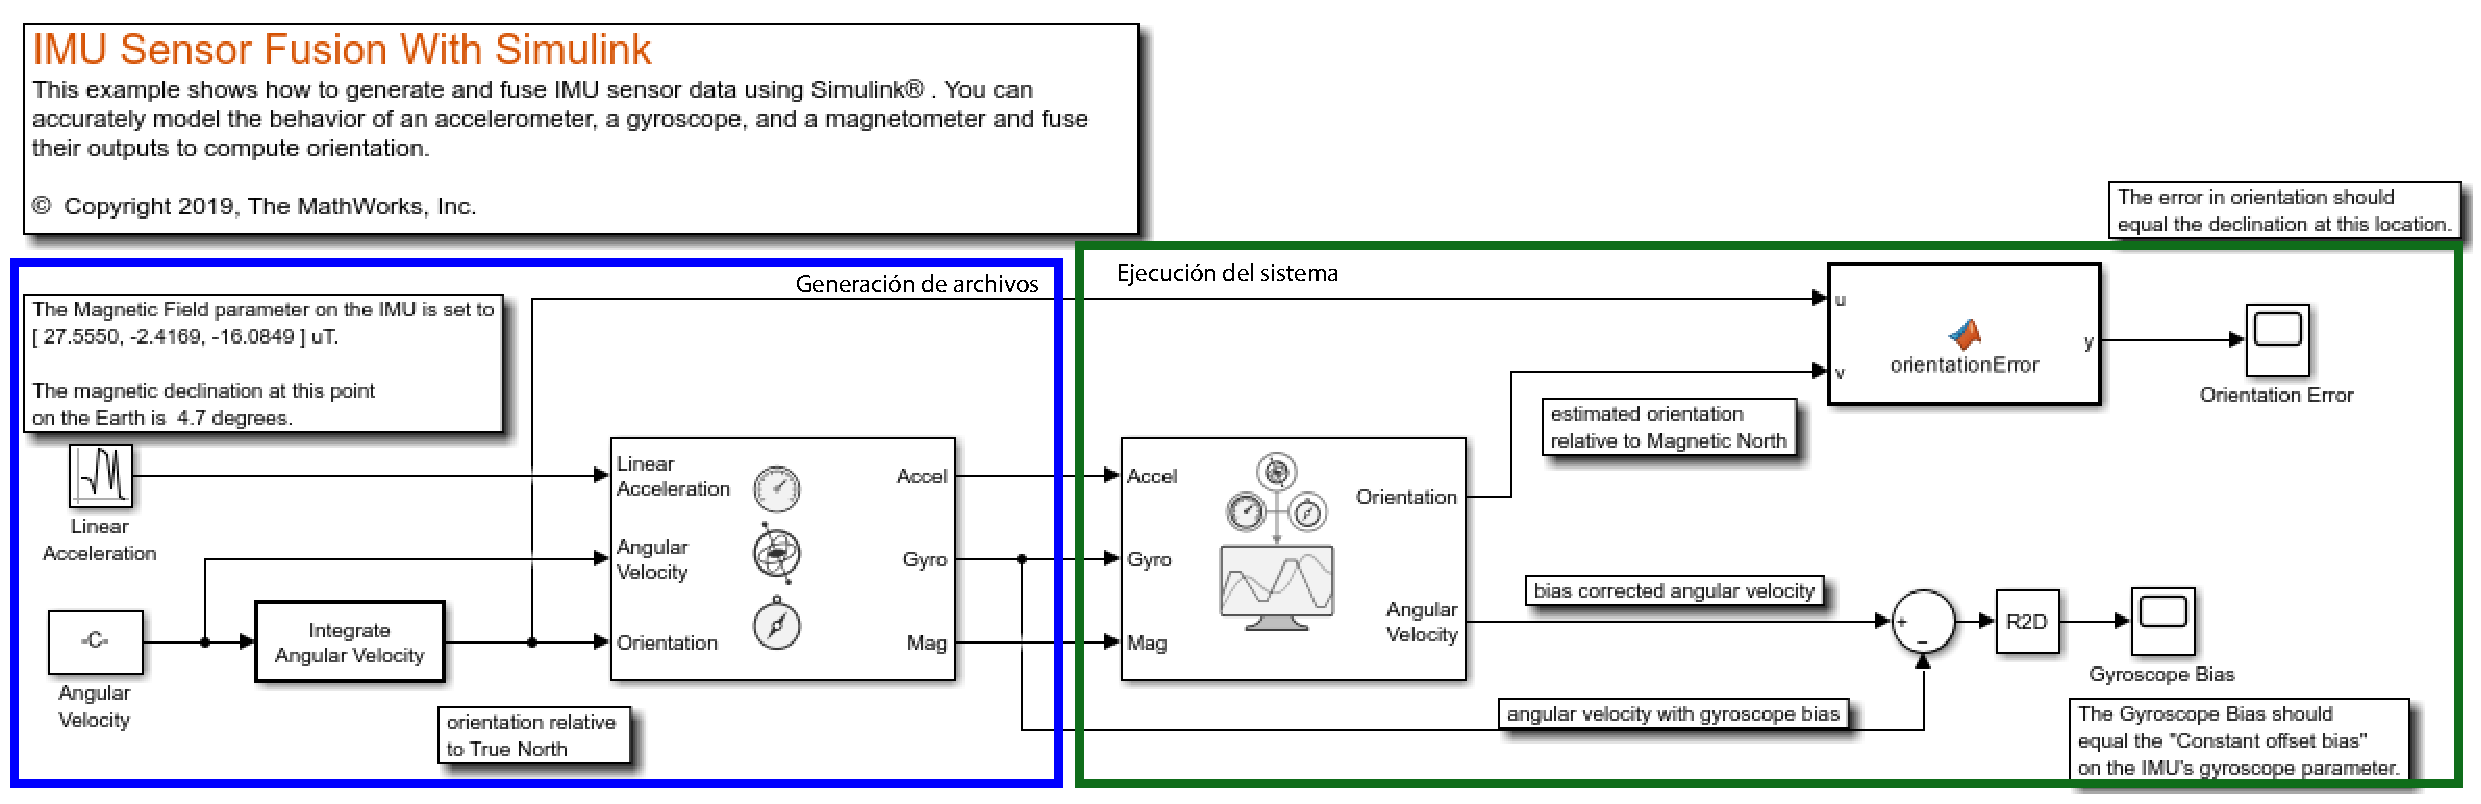
\includegraphics[width=1.0\textwidth]{fig/Capitulo5/Caso_de_estudio_IMU/FULL_IMU.pdf}
    \caption{Diagrama completo del caso de estudio 2 - IMU \cite{mathworks2024imu}}
    \label{fig:caso_de_estudio_2_IMU}
\end{figure}


Como se observa en la Figura \ref{fig:caso_de_estudio_2_IMU}, este es el caso de estudio que se propuso en \cite{mathworks2024imu}, se le deben de realizar unas modificaciones de acuerdo al funcionamiento deseado, siempre generando datos en el ámbito de simulación en MATLAB para luego contrastar los mismos con los datos obtenidos en la ejecución del modelo en la tarjeta de desarrollo seleccionada.

\subsection{Bloques utilizados para la implementación}

Los bloques utilizados se obtuvieron en la librería de bloques de MATLAB Simulink. A continuación se muestran los bloques utilizados, así como la configuración empleada en los mismos para la correcta operación del modelo. La implementación del sistema se dividió en dos partes. La primera parte se encargó de generar los archivos necesarios para la operación del sistema mientras que la segunda parte del sistema, tomo los archivos de datos y se encargó de leerlos archivos con los datos y generar los dos archivos de salida del programa.

\subsubsection{Sistema para la generación de archivos}\label{subsub:generación_de_archivos}

\begin{figure}[h!]
    \centering
    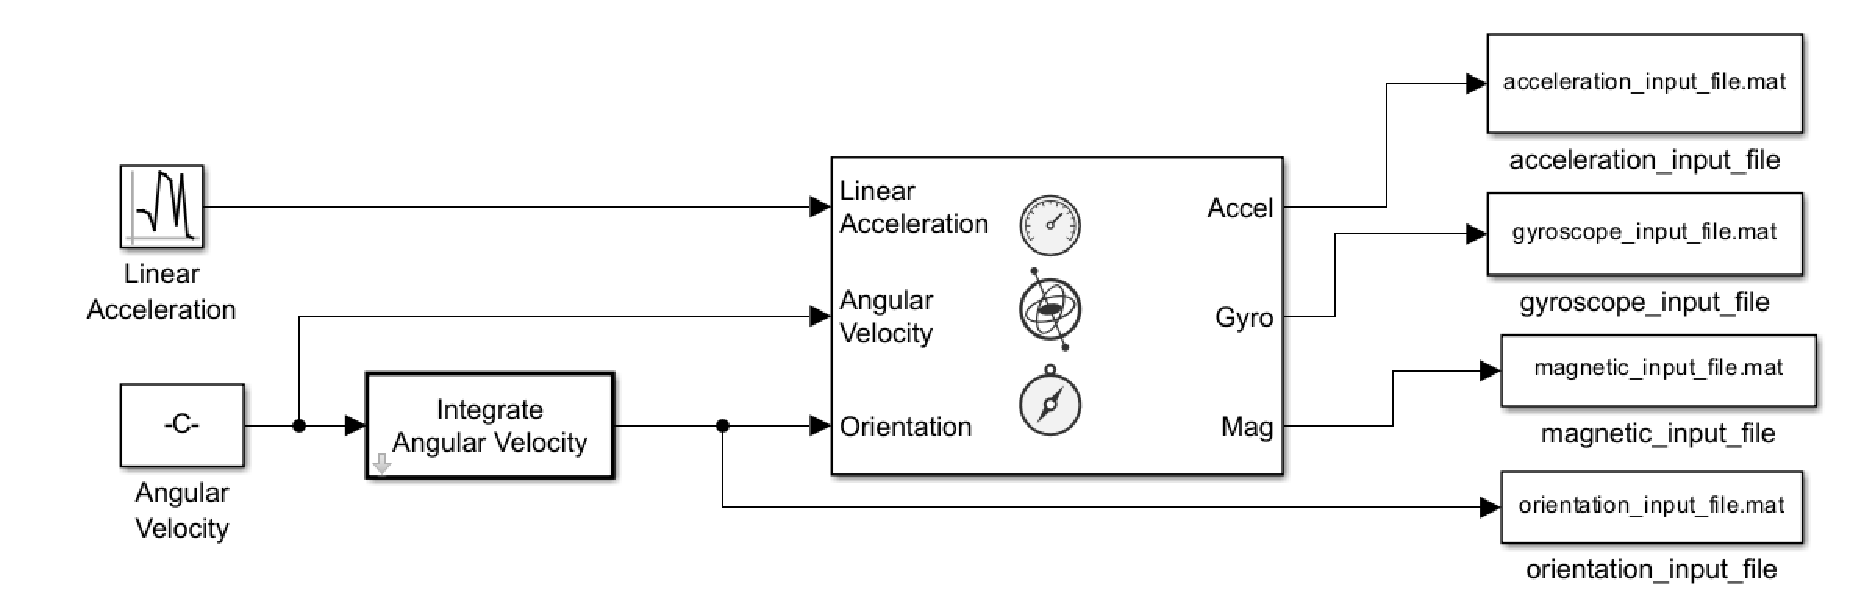
\includegraphics[width=0.8\textwidth]{fig/Capitulo5/Caso_de_estudio_IMU/Generador_de_archivos/flujo_generador_de_archivos.pdf}
    \caption{Diagrama utilizado para la generación de los archivos \cite{mathworks2024imu}}
    \label{fig:caso_de_estudio_2_IMU_generación_de_archivos}
\end{figure}

Este sistema fue el encargado de generar los archivos de entrada, estos contenían los datos de tiempo y valores para la correcta implementación del sistema, los bloques se utilizaron para construir el diagrama de la Figura \ref{fig:caso_de_estudio_2_IMU_generación_de_archivos}.

\begin{figure}[htbp]
    \centering
    \begin{subfigure}[b]{0.45\textwidth}
        \centering
        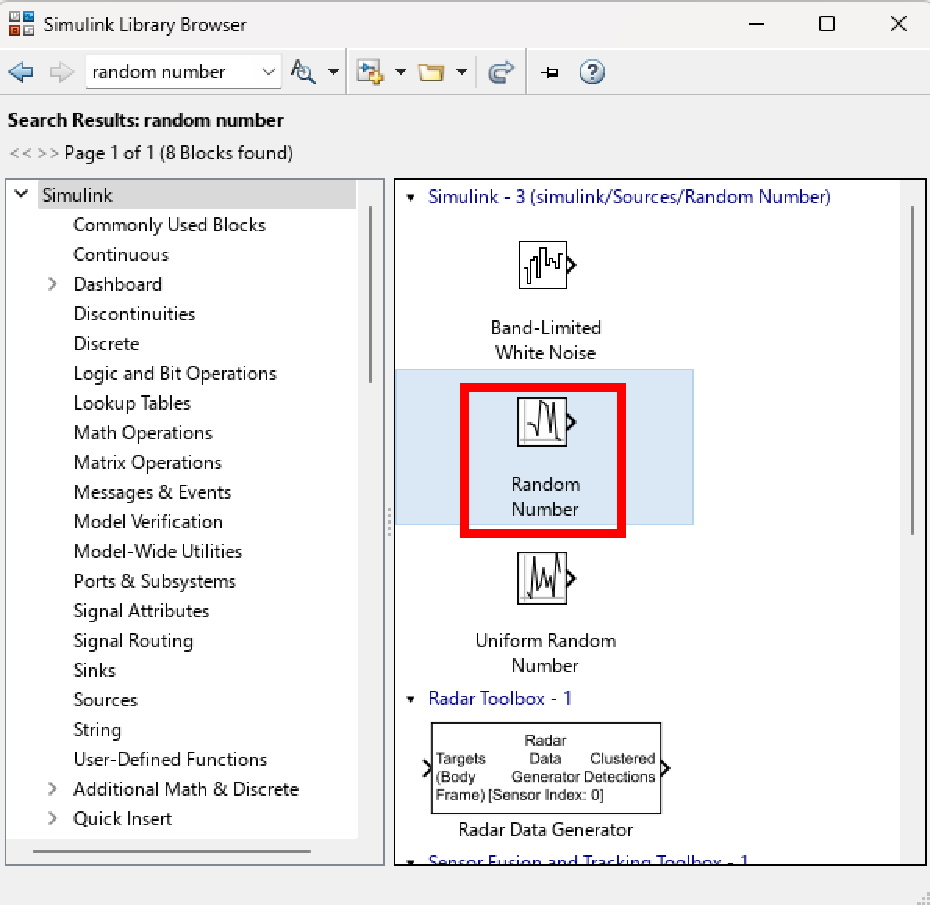
\includegraphics[width=\textwidth]{fig/Capitulo5/Caso_de_estudio_IMU/Generador_de_archivos/libreria_de_bloques_aceleracion_lineal.pdf}
        \caption{Librería de bloques - Aceleración Lineal}
        \label{fig:lib_bloques_linear_acceleration}
    \end{subfigure}
    \hfill
    \begin{subfigure}[b]{0.45\textwidth}
        \centering
        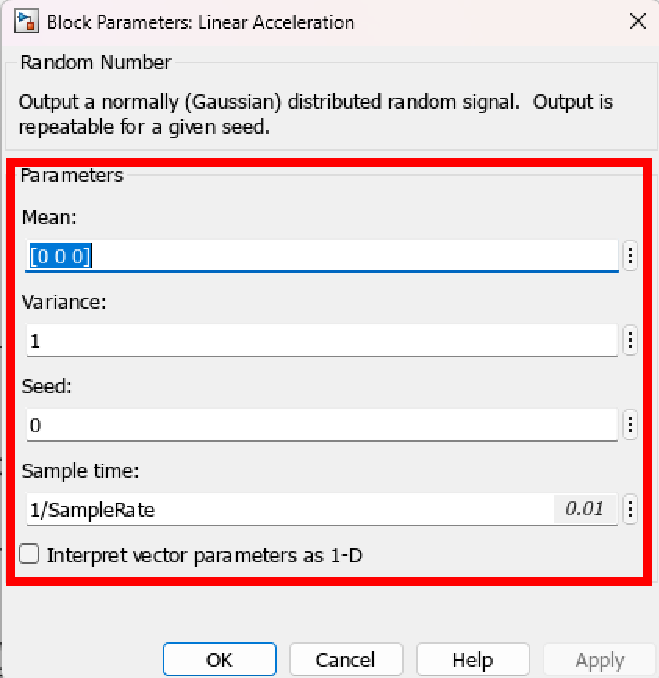
\includegraphics[width=\textwidth]{fig/Capitulo5/Caso_de_estudio_IMU/Generador_de_archivos/configuracion_bloque_aceleracion_lineal.pdf}
        \caption{Configuración del bloque aceleración lineal}
        \label{fig:lib_bloques_config_linear_acceleration}
    \end{subfigure}
    \caption{Bloque para la aceleración lineal}
    \label{fig:linear_accel_block_simulink}
\end{figure}

Como se observa en la Figura \ref{fig:linear_accel_block_simulink}, se presenta a la izquierda la librería donde se encuentra el bloque a utilizar para establecer la constante de la velocidad angular, para este caso se utilizó en el mismo el valor que se observa en la Figura \ref{fig:lib_bloques_config_linear_acceleration}, además de algunas configuraciones adicionales requeridas por el bloque. 

\begin{figure}[htbp]
    \centering
    \begin{subfigure}[b]{0.45\textwidth}
        \centering
        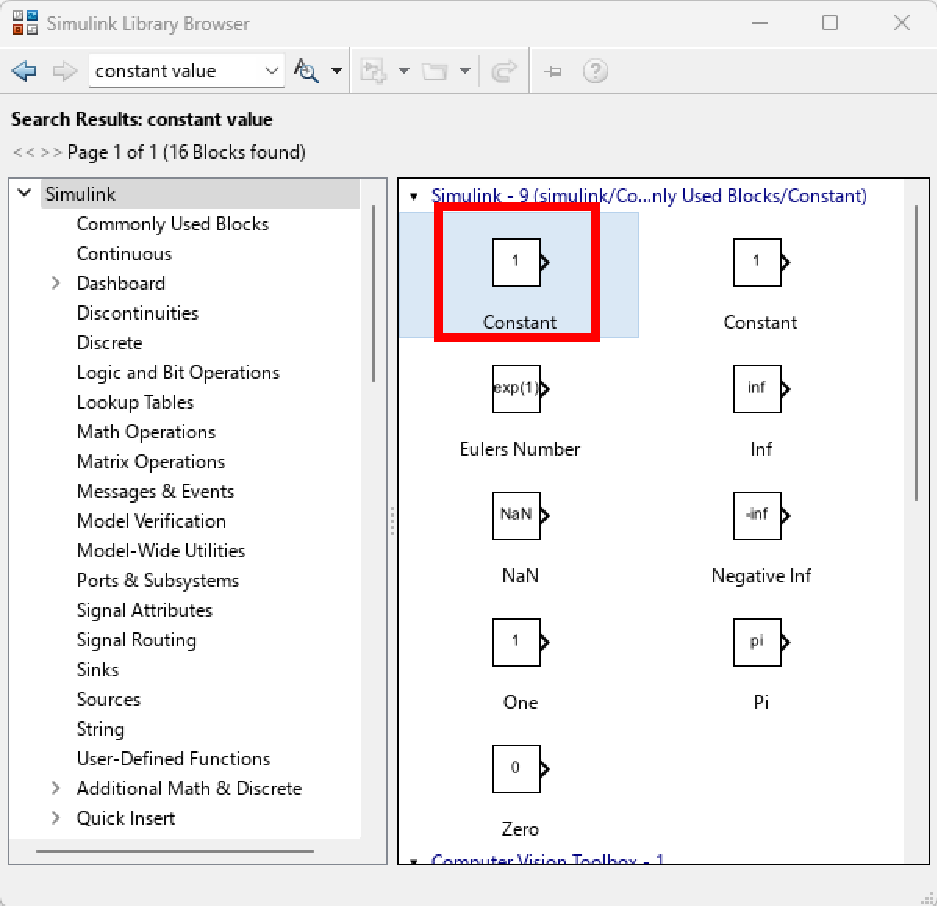
\includegraphics[width=\textwidth]{fig/Capitulo5/Caso_de_estudio_IMU/Generador_de_archivos/libreria_de_bloques_constante_velocidad_angular.pdf}
        \caption{Librería de bloques - Velocidad Angular}
        \label{fig:lib_bloques_angular_velocity}
    \end{subfigure}
    \hfill
    \begin{subfigure}[b]{0.45\textwidth}
        \centering
        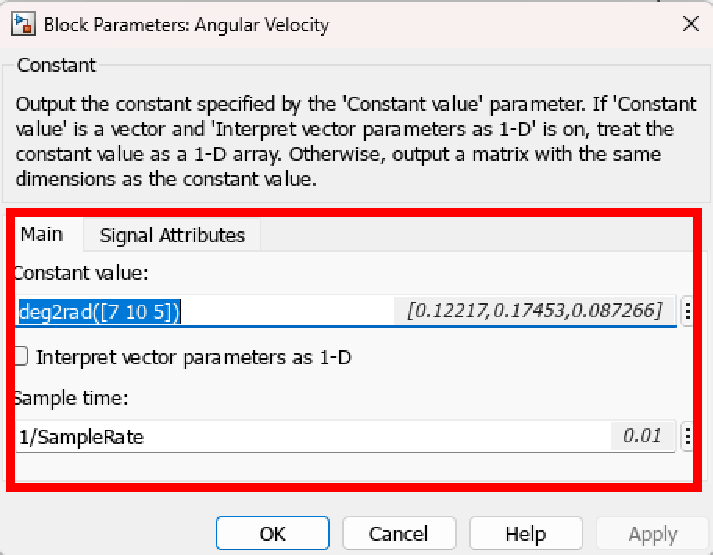
\includegraphics[width=\textwidth]{fig/Capitulo5/Caso_de_estudio_IMU/Generador_de_archivos/configuracion_bloque_velocidad_angular.pdf}
        \caption{Configuración del bloque velocidad angular}
        \label{fig:lib_bloques_config_angular_velocity}
    \end{subfigure}
    \caption{Bloque para la velocidad angular}
    \label{fig:angular_velocity_block_simulink}
\end{figure}

Seguido de esto, en la Figura \ref{fig:angular_velocity_block_simulink} se observa el bloque encargado de establecer la variable de la velocidad angular, a la izquierda el bloque a utilizar en la librería y a la derecha se encuentra la configuración utilizada para este bloque. 

\newpage

\begin{figure}[htbp]
    \centering
    \begin{subfigure}[b]{0.35\textwidth}
        \centering
        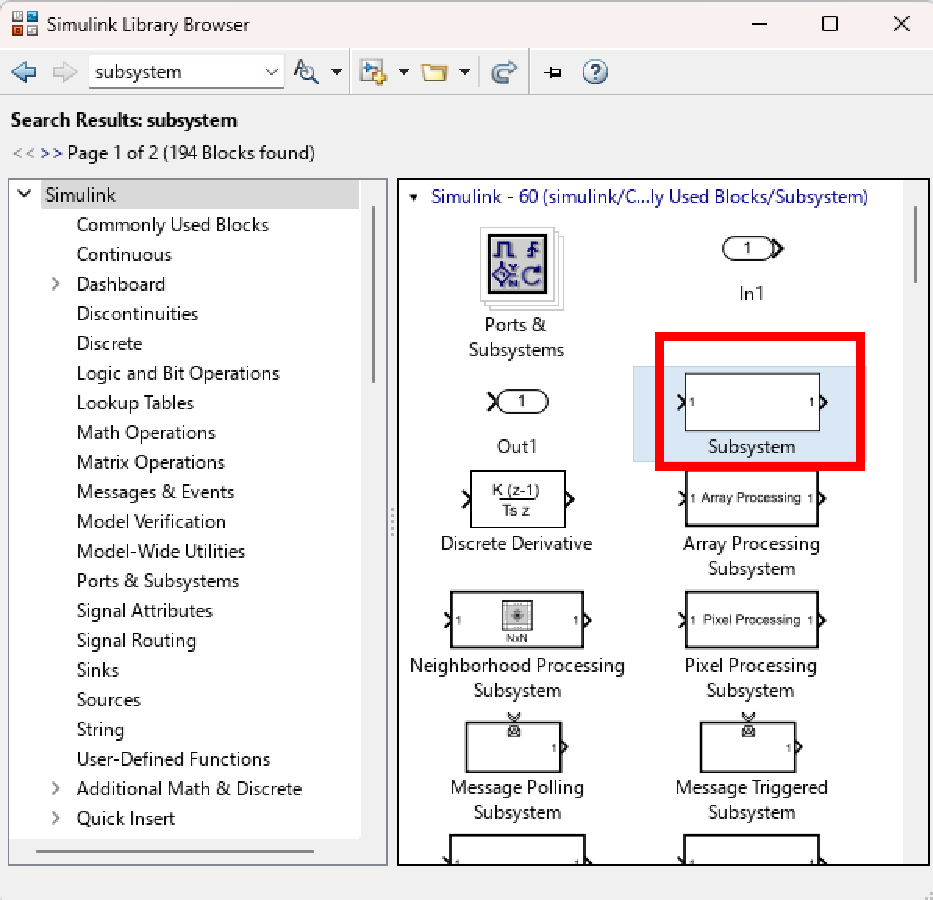
\includegraphics[width=\textwidth]{fig/Capitulo5/Caso_de_estudio_IMU/Generador_de_archivos/libreria_de_bloques_subsistema_integracion_velocidad_angular.pdf}
        \caption{Librería de bloques - Integrador}
        \label{fig:lib_bloques_integrador}
    \end{subfigure}
    \hfill
    \begin{subfigure}[b]{0.45\textwidth}
        \centering
        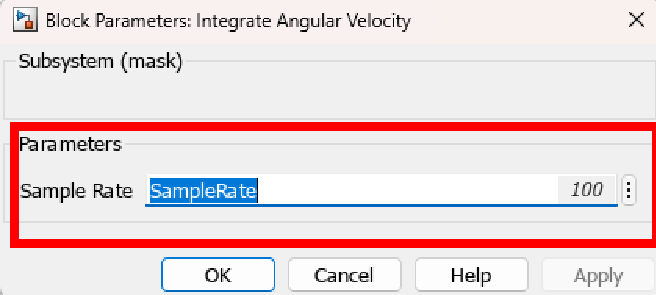
\includegraphics[width=\textwidth]{fig/Capitulo5/Caso_de_estudio_IMU/Generador_de_archivos/configuracion_integrador_velocidad_angular.pdf}
        \caption{Configuración del bloque velocidad angular}
        \label{fig:config_bloques_integrador}
    \end{subfigure}
    \caption{Bloque para la integración de la velocidad angular}
    \label{fig:integration_for_angular_velocity}
\end{figure}

Adicional al bloque que se muestra en \ref{fig:angular_velocity_block_simulink} también se implementó un bloque encargado de integrar el valor de la velocidad angular, para esto se usa el bloque que se muestra en la Figura \ref{fig:integration_for_angular_velocity}, este mismo se encontró en la librería de bloques de Simulink como se muestra en \ref{fig:lib_bloques_integrador}, también, en la Figura \ref{fig:config_bloques_integrador} se muestran los parámetros que se utilizaron en la configuración del bloque.
\newpage

\begin{figure}[htbp]
    \centering
    % Primera imagen
    \begin{subfigure}[b]{0.35\textwidth}
        \centering
        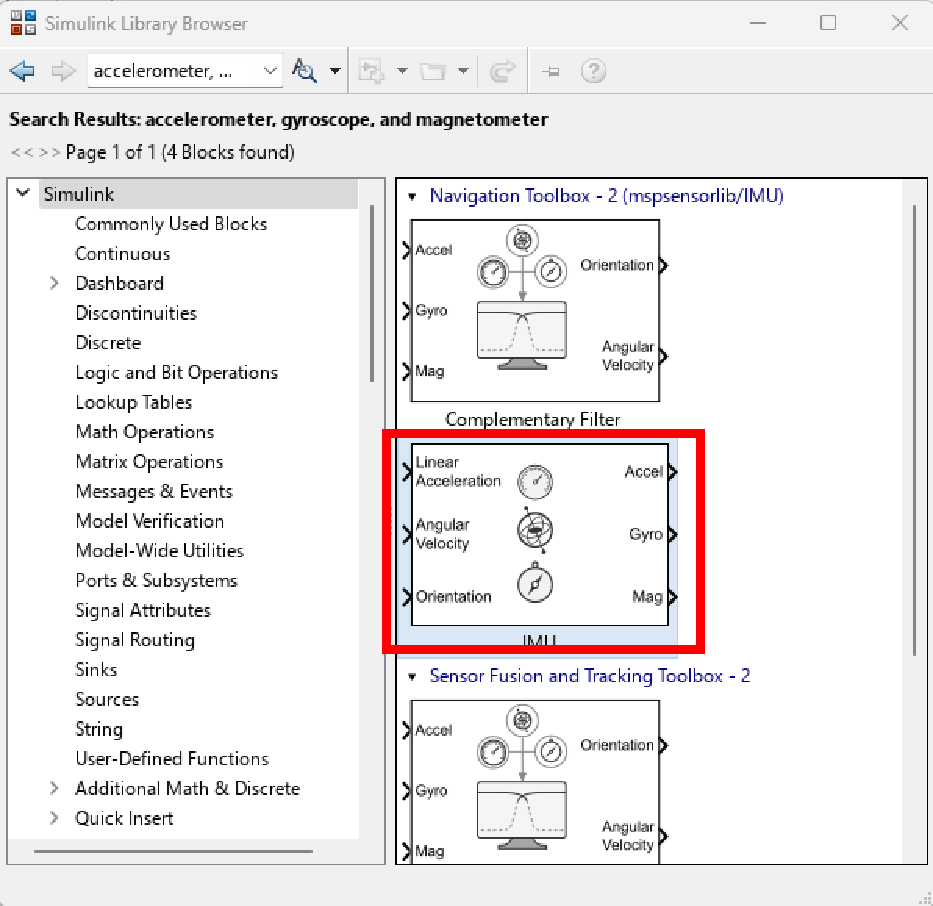
\includegraphics[width=\textwidth]{fig/Capitulo5/Caso_de_estudio_IMU/Generador_de_archivos/libreria_de_bloques_IMU.pdf}
        \caption{Librería de bloques - IMU}
        \label{fig:lib_bloques_IMU}
    \end{subfigure}
    \hfill
    % Segunda imagen
    \begin{subfigure}[b]{0.35\textwidth}
        \centering
        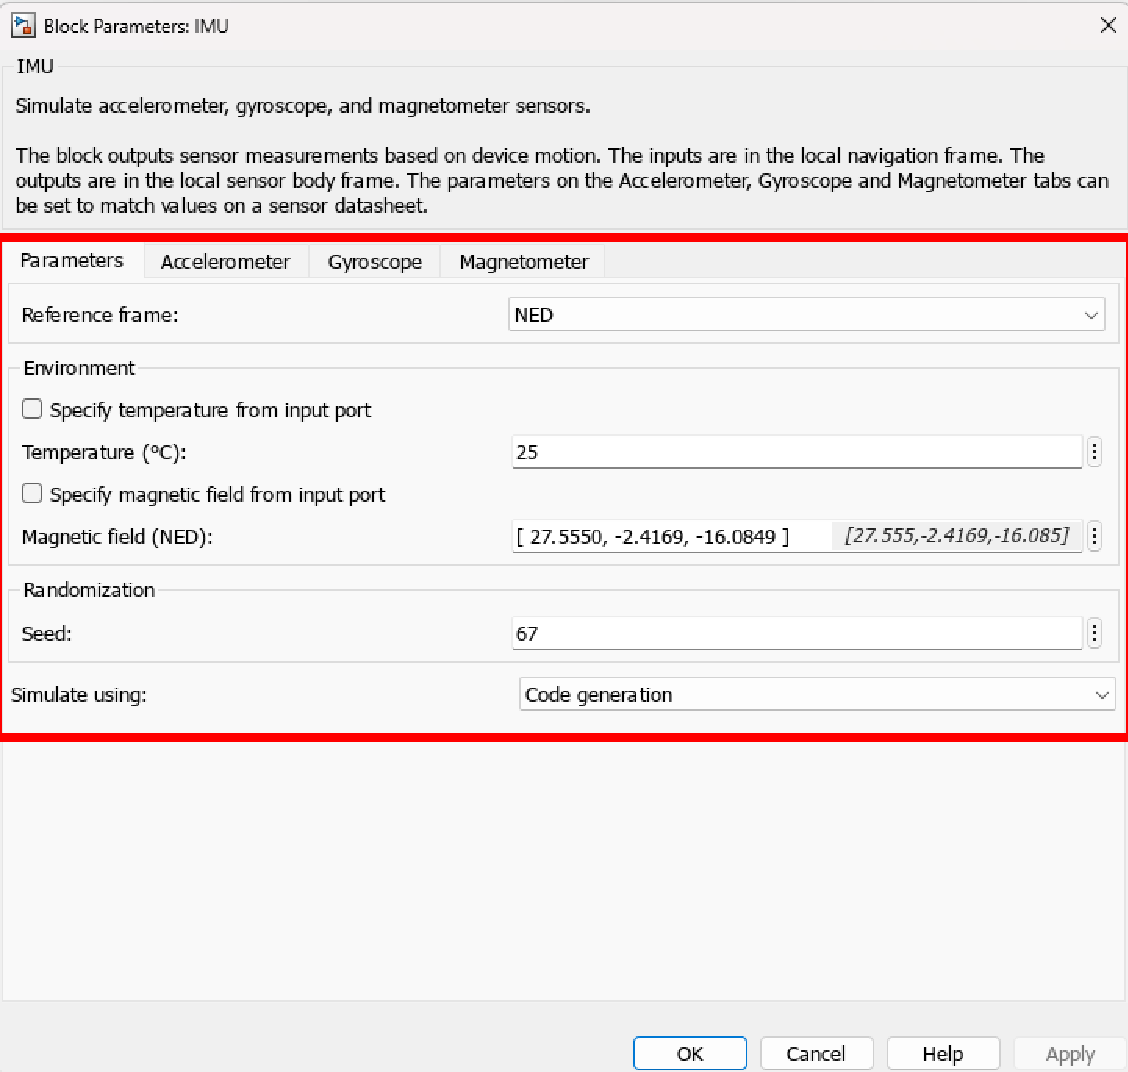
\includegraphics[width=\textwidth]{fig/Capitulo5/Caso_de_estudio_IMU/Generador_de_archivos/configuracion_parametros_IMU_01.pdf}
        \caption{Configuración de parámetros 1}
        \label{fig:parametros_IMU_01}
    \end{subfigure}
    \hfill
    % Tercera imagen
    \begin{subfigure}[b]{0.35\textwidth}
        \centering
        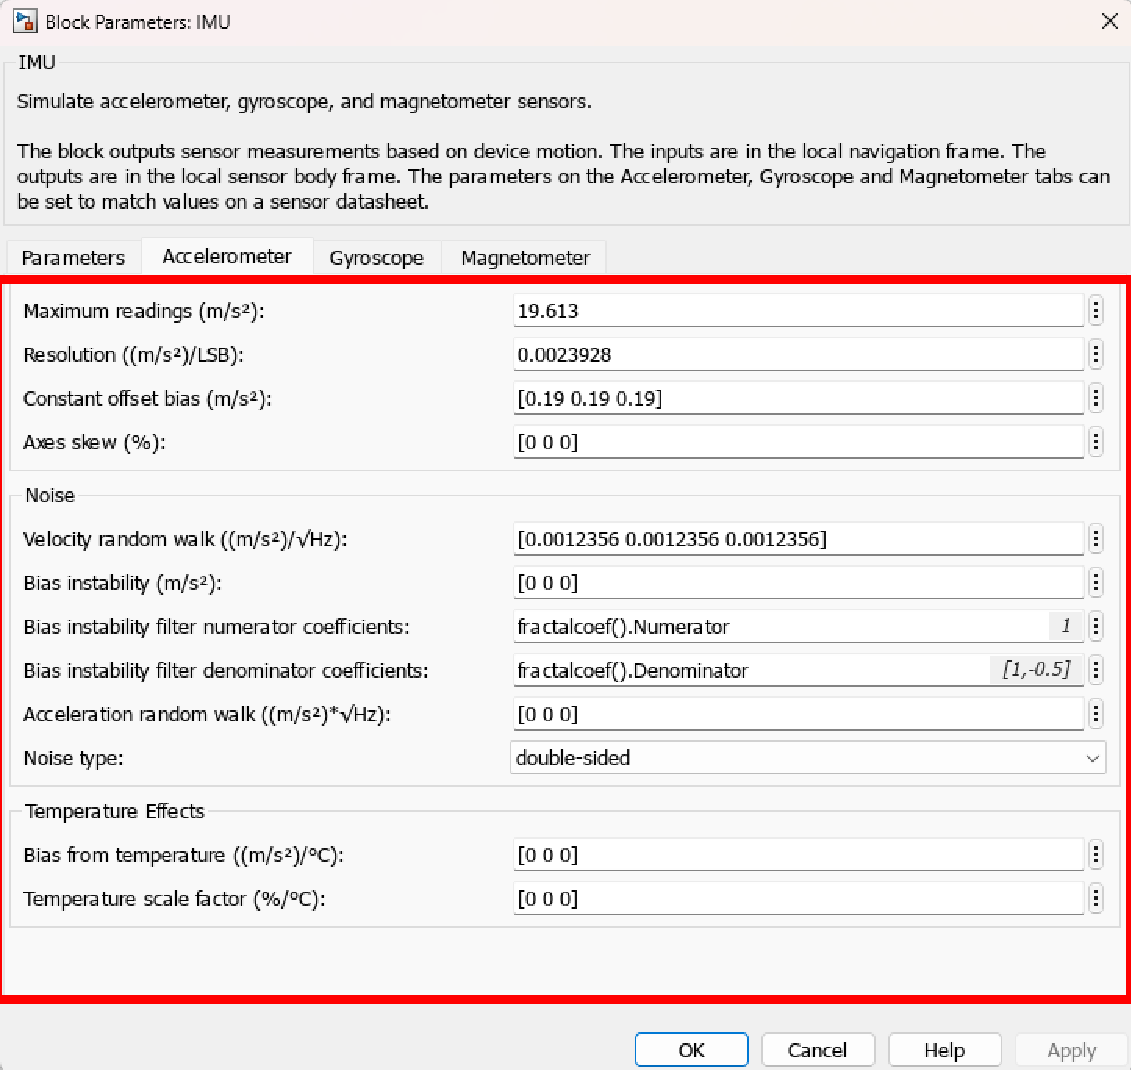
\includegraphics[width=\textwidth]{fig/Capitulo5/Caso_de_estudio_IMU/Generador_de_archivos/configuracion_parametros_IMU_02.pdf}
        \caption{Configuración de parámetros 2}
        \label{fig:parametros_IMU_02}
    \end{subfigure}
    \hfill
    % Cuarta imagen
    \begin{subfigure}[b]{0.35\textwidth}
        \centering
        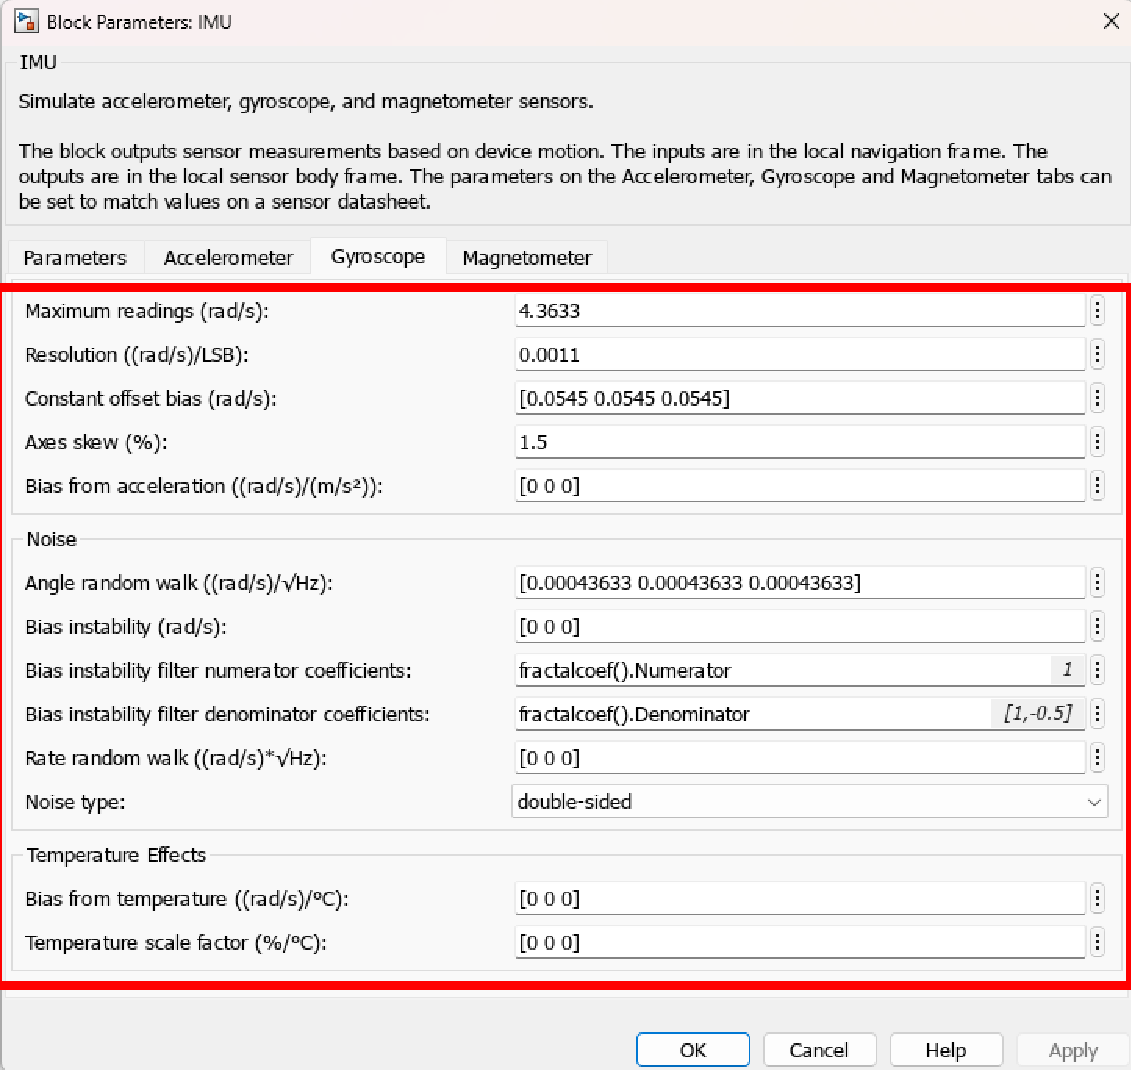
\includegraphics[width=\textwidth]{fig/Capitulo5/Caso_de_estudio_IMU/Generador_de_archivos/configuracion_parametros_IMU_03.pdf}
        \caption{Configuración de parámetros 3}
        \label{fig:parametros_IMU_03}
    \end{subfigure}
    \hfill
    % Quinta imagen
    \begin{subfigure}[b]{0.35\textwidth}
        \centering
        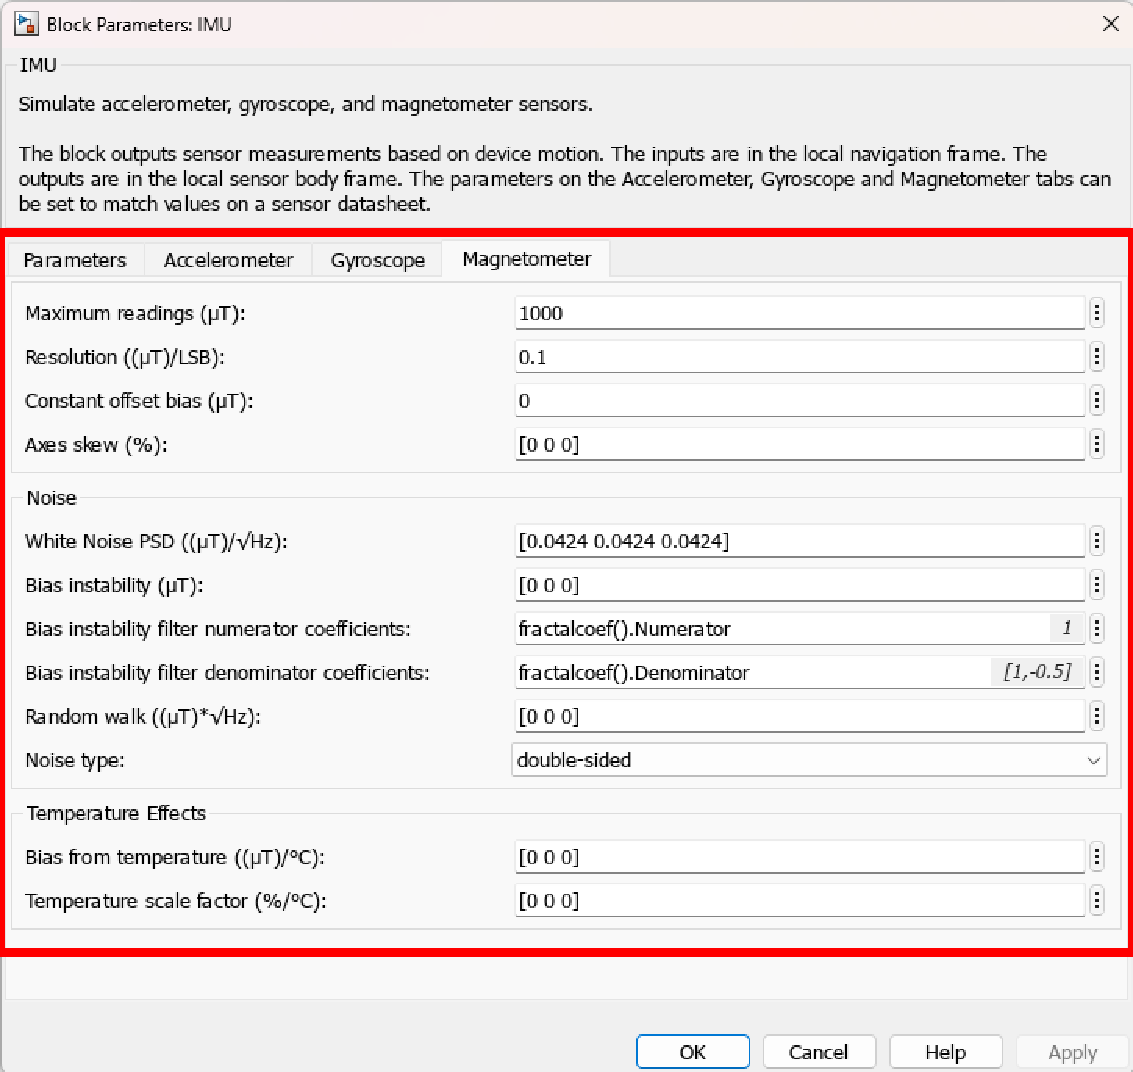
\includegraphics[width=\textwidth]{fig/Capitulo5/Caso_de_estudio_IMU/Generador_de_archivos/configuracion_parametros_IMU_04.pdf}
        \caption{Configuración de parámetros 4}
        \label{fig:parametros_IMU_04}
    \end{subfigure}

    \caption{Bloque para la simulación del comportamiento de la IMU}
    \label{fig:arreglo_imu}
\end{figure}


Finalmente en la Figura \ref{fig:arreglo_imu} se presenta el bloque que se encargó de simular la detección y medición de la aceleración y rotación en diferentes ejes de un sistema. Por un lado en la Figura \ref{fig:lib_bloques_IMU} se muestra el bloque en la librería. Por otro lado, en la Figura \ref{fig:parametros_IMU_01} la configuración del bloque respecto a los parámetros del mismo, esto contemplo desde el marco de referencia a utilizar, la temperatura de operación del sistema, las componentes del campo magnético y la semilla, en la Figura \ref{fig:parametros_IMU_02} la configuración utilizada en el bloque para las componentes relacionadas con el acelerómetro, las mismas contemplan desde la configuración de máximos de lectura, resolución del sensor, el ruido y los efectos de temperatura, en la Figura \ref{fig:parametros_IMU_03} se presenta la configuración del boque relacionada con los parámetros del giroscopio, estos contemplan algunos parámetros similares a los del acelerómetro y finalmente en la Figura \ref{fig:parametros_IMU_04} se muestra la configuración empleada para el magnetómetro. Cabe destacar que si se quiere replicar el experimento se deben de usar los parámetros mostrados en las imágenes contenidas en \ref{fig:arreglo_imu}. 


\begin{figure}[htbp]
    \centering
    \begin{subfigure}[b]{0.35\textwidth}
        \centering
        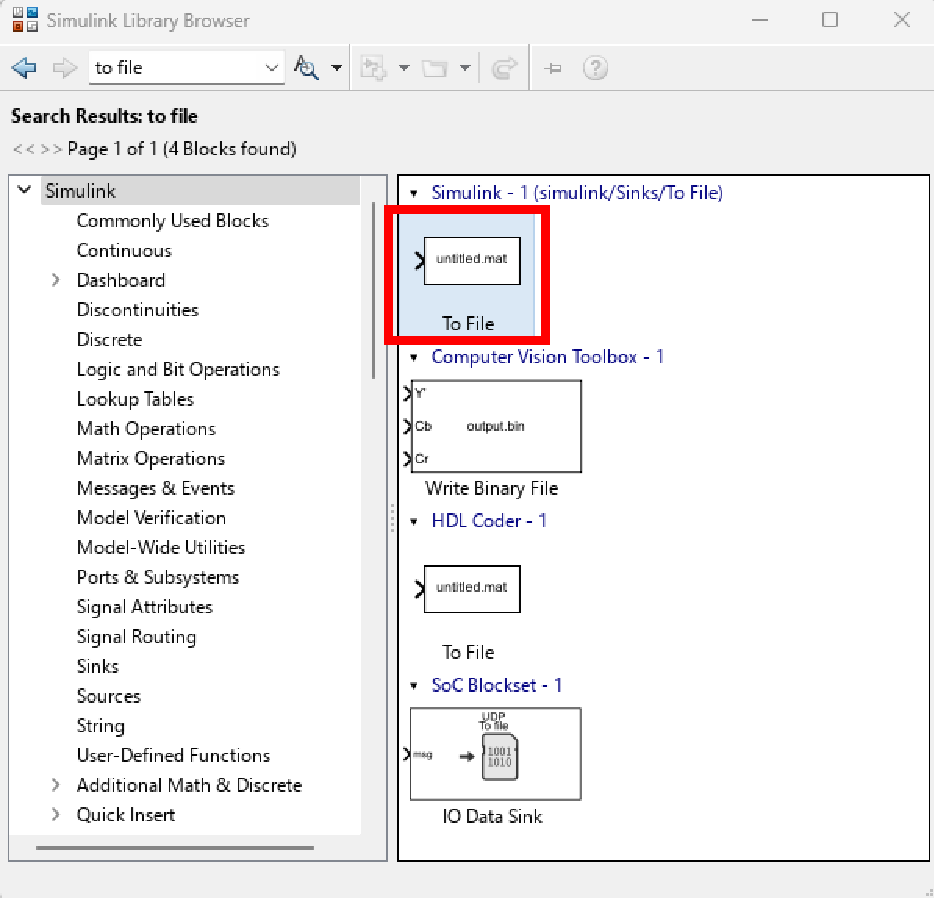
\includegraphics[width=\textwidth]{fig/Capitulo5/Caso_de_estudio_IMU/Generador_de_archivos/libreria_de_bloques_to_file.pdf}
        \caption{Librería de bloques - Guardar en archivo}
        \label{fig:lib_bloques_to_file_IMU}
    \end{subfigure}
    \hfill
    \begin{subfigure}[b]{0.45\textwidth}
        \centering
        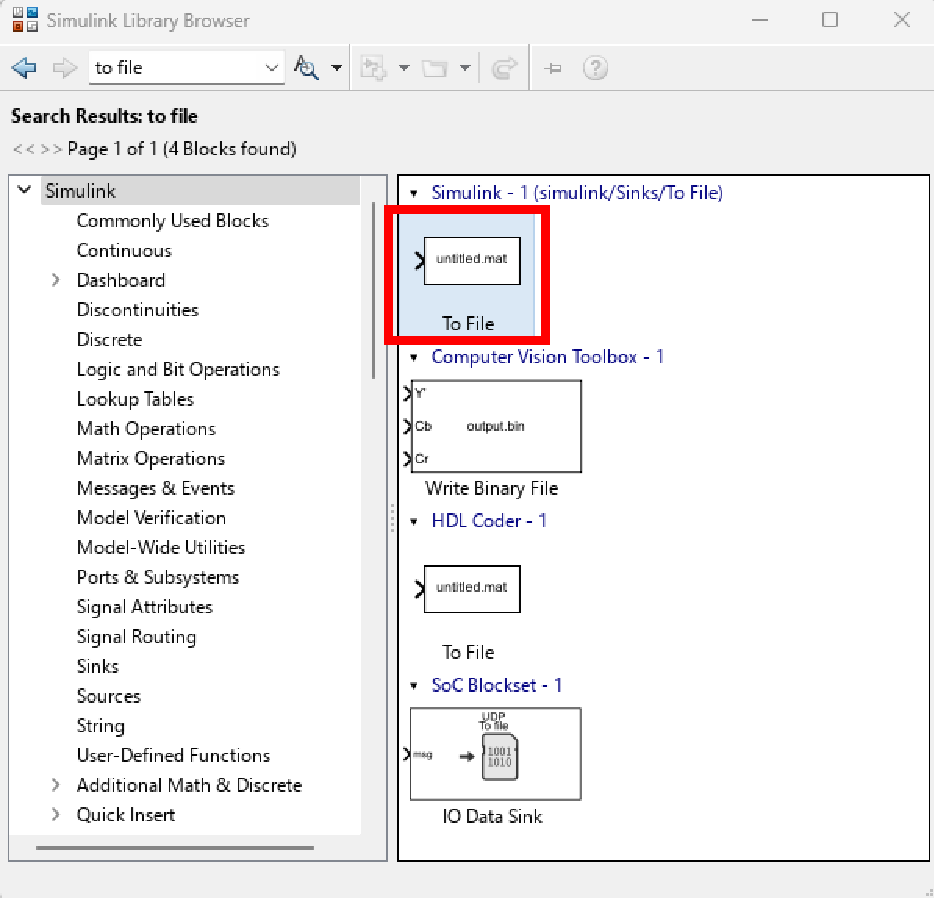
\includegraphics[width=\textwidth]{fig/Capitulo5/Caso_de_estudio_IMU/Generador_de_archivos/libreria_de_bloques_to_file.pdf}
        \caption{Configuración de parámetros - Guardar en archivo}
        \label{fig:config_to_file_IMU}
    \end{subfigure}
    \caption{Bloque para guardar los datos en un archivo}
    \label{fig:to_file_IMU}
\end{figure}

Para  generar archivos los cuales se utilizaron más adelante en este caso de estudio se utilizó el bloque que se muestra en la Figura \ref{fig:to_file_IMU}, este se encargó de generar un archivo en formato (.mat) con el objetivo de proveer datos a las otras secciones de este caso de estudio, cabe destacar que la configuración del mismo se muestra en la Figura \ref{fig:config_to_file_IMU} en donde se establece el nombre del archivo de salida, la forma de almacenamiento de los datos y finalmente el nombre de la variable por la cual se accederán estos datos. Los nombres a utilizar son:

\begin{itemize}
    \item acceleration\_input\_file
    \item gyroscope\_input\_file
    \item magnetic\_input\_file
    \item orientation\_input\_file
\end{itemize}

Estos nombres se deben de respetar a la hora de generar los archivos de salida, ya que el programa encargado de recibir estos datos buscara los archivos en el directorio bajo estos nombres.

\newpage

\subsubsection{Sistema para la lectura e interpretación de los archivos generados previamente}

\begin{figure}[h!]
    \centering
    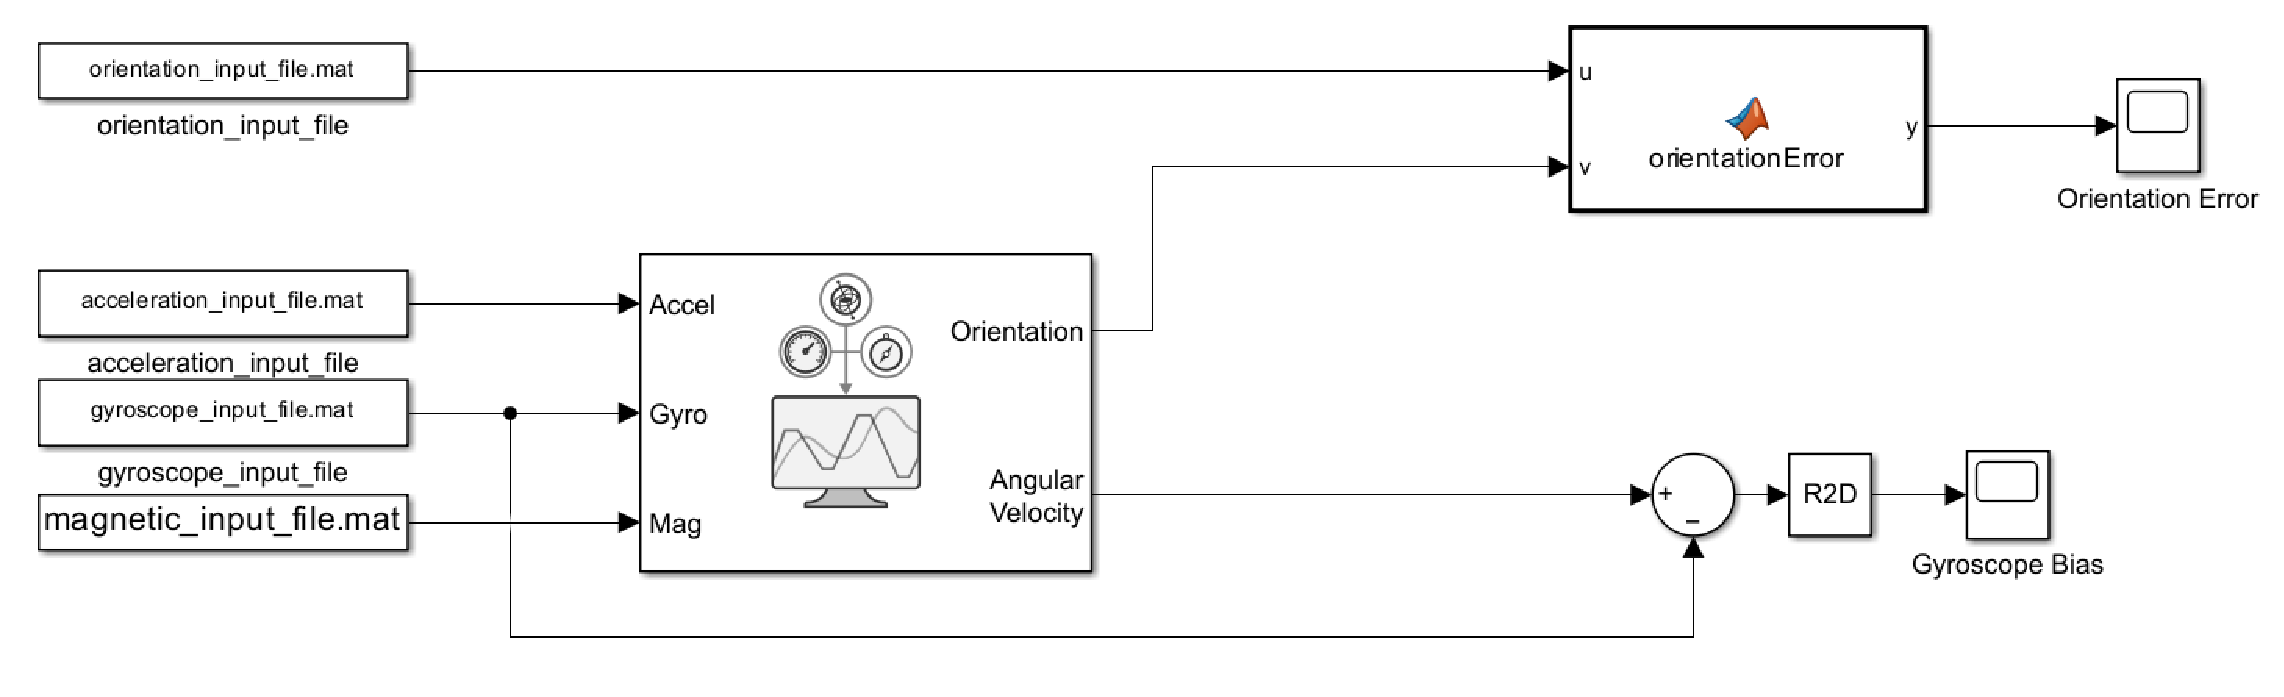
\includegraphics[width=0.8\textwidth]{fig/Capitulo5/Caso_de_estudio_IMU/Generador_de_salidas/flujo_lector_de_archivos.pdf}
    \caption{Diagrama utilizado para la interpretación de los archivos \cite{mathworks2024imu}}
    \label{fig:caso_de_estudio_2_IMU_interpretacion_de_archivos}
\end{figure}


Una vez fue establecido el diagrama que se encarga de la generación de los datos, en esta sección se explican los bloques requeridos para la construcción del diagrama de la Figura \ref{fig:caso_de_estudio_2_IMU_interpretacion_de_archivos}.

\begin{figure}[htbp]
    \centering
    \begin{subfigure}[b]{0.35\textwidth}
        \centering
        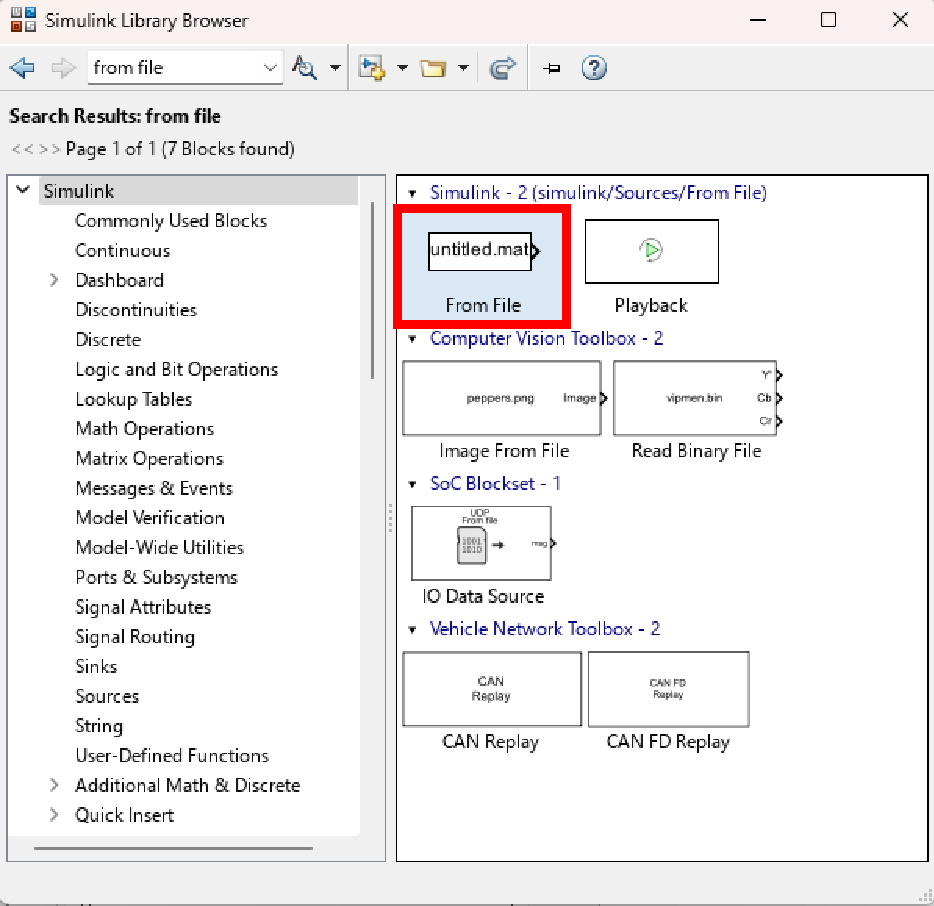
\includegraphics[width=\textwidth]{fig/Capitulo5/Caso_de_estudio_IMU/Generador_de_salidas/libreia_de_bloques_from_file.pdf}
        \caption{Librería de bloques - Leer de archivo}
        \label{fig:lib_bloques_from_file_IMU}
    \end{subfigure}
    \hfill
    \begin{subfigure}[b]{0.45\textwidth}
        \centering
        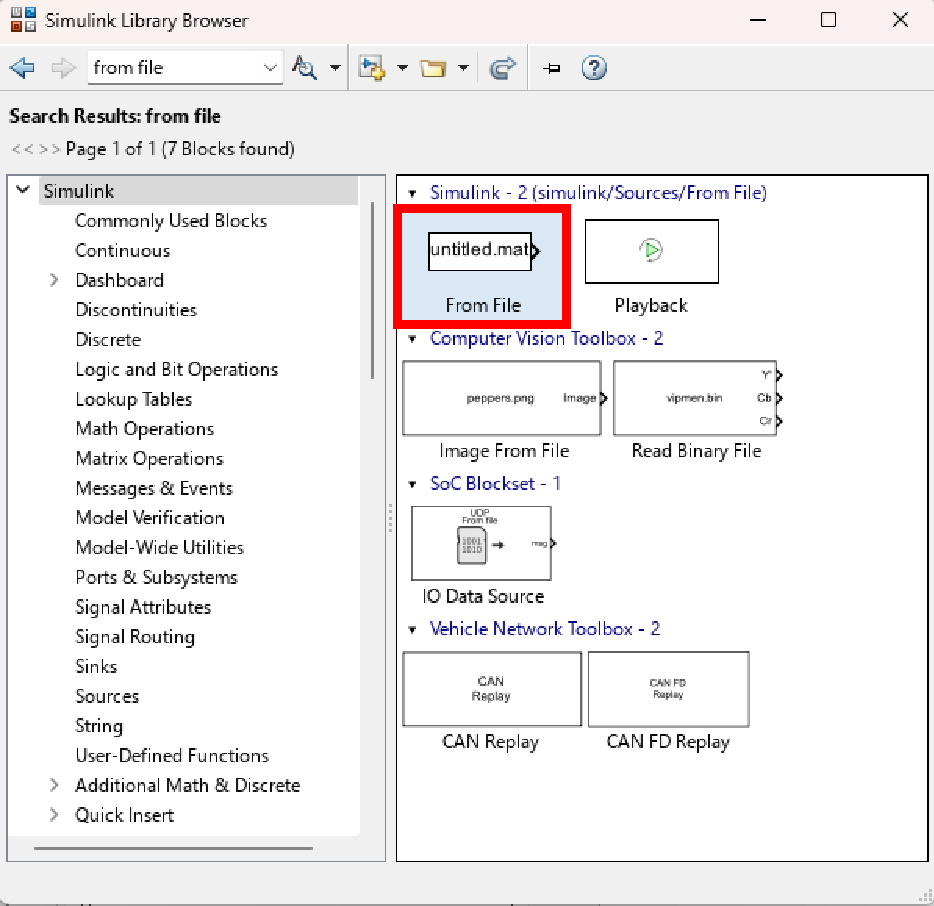
\includegraphics[width=\textwidth]{fig/Capitulo5/Caso_de_estudio_IMU/Generador_de_salidas/libreia_de_bloques_from_file.pdf}
        \caption{Configuración del bloque encargado de la lectura de archivos}
        \label{fig:config_from_file_IMU}
    \end{subfigure}
    \caption{Bloque para la lectura de archivos}
    \label{fig:read_from_file}
\end{figure}

El desarrollo de este capítulo, en \ref{subsub:generación_de_archivos} se tuvo como salida del programa una serie de archivos generados. Para  leer los archivos generados previamente se utilizó del bloque que se muestra en la Figura \ref{fig:read_from_file}, para el correcto funcionamiento del sistema es muy importante que los parámetros de configuración que se muestran en la Figura \ref{fig:config_from_file_IMU}.
\newpage

\begin{figure}[htbp]
    \centering
    % Primera imagen
    \begin{subfigure}[b]{0.35\textwidth}
        \centering
        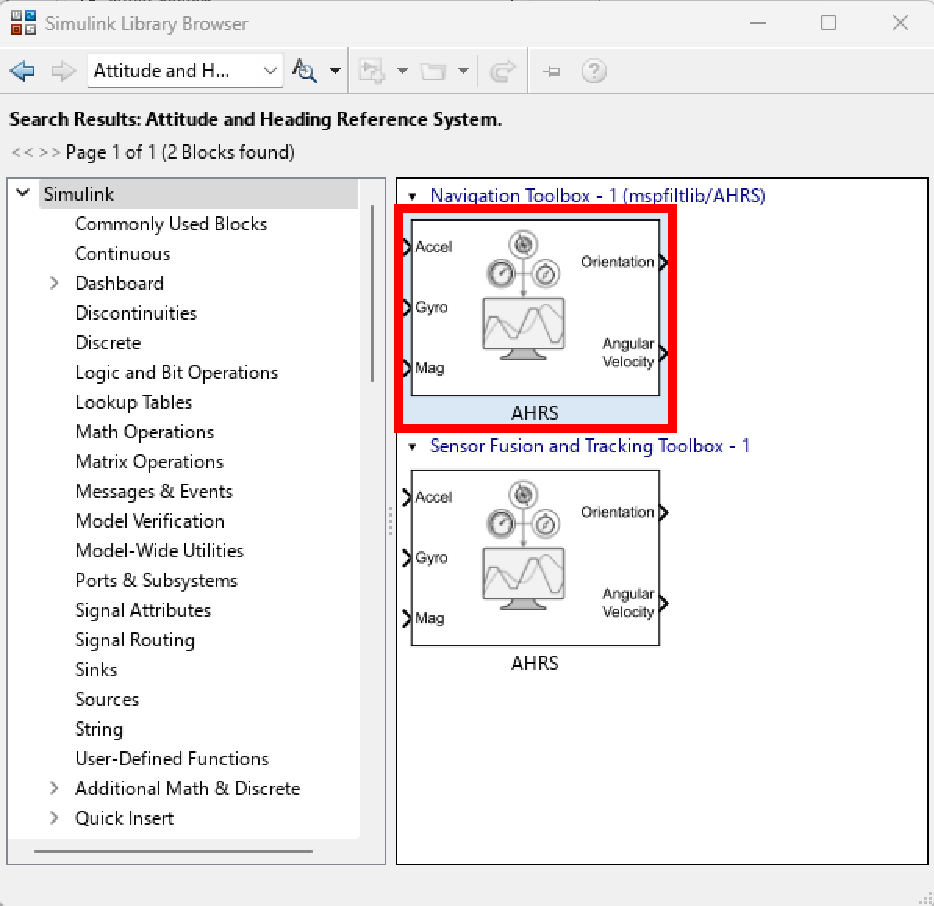
\includegraphics[width=\textwidth]{fig/Capitulo5/Caso_de_estudio_IMU/Generador_de_salidas/libreira_de_bloques_sensor_AHRS.pdf}
        \caption{Librería de bloques - AHRS}
        \label{fig:lib_bloques_AHRS}
    \end{subfigure}
    \hfill
    % Segunda imagen
    \begin{subfigure}[b]{0.45\textwidth}
        \centering
        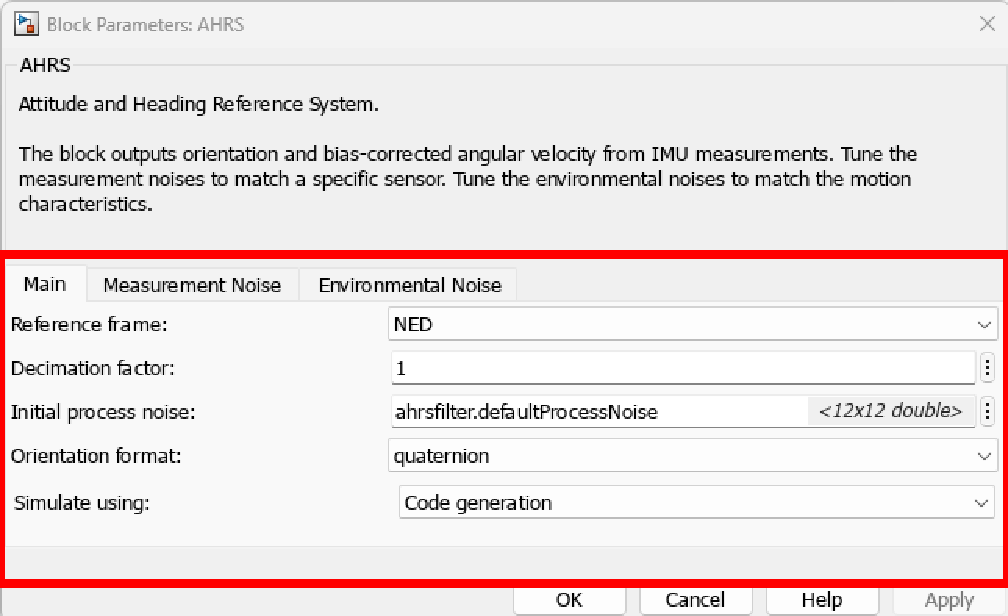
\includegraphics[width=\textwidth]{fig/Capitulo5/Caso_de_estudio_IMU/Generador_de_salidas/configuracion_AHRS_01.pdf}
        \caption{Configuración de parámetros 1}
        \label{fig:parametros_AHRS_01}
    \end{subfigure}
    \hfill
    % Tercera imagen
    \begin{subfigure}[b]{0.45\textwidth}
        \centering
        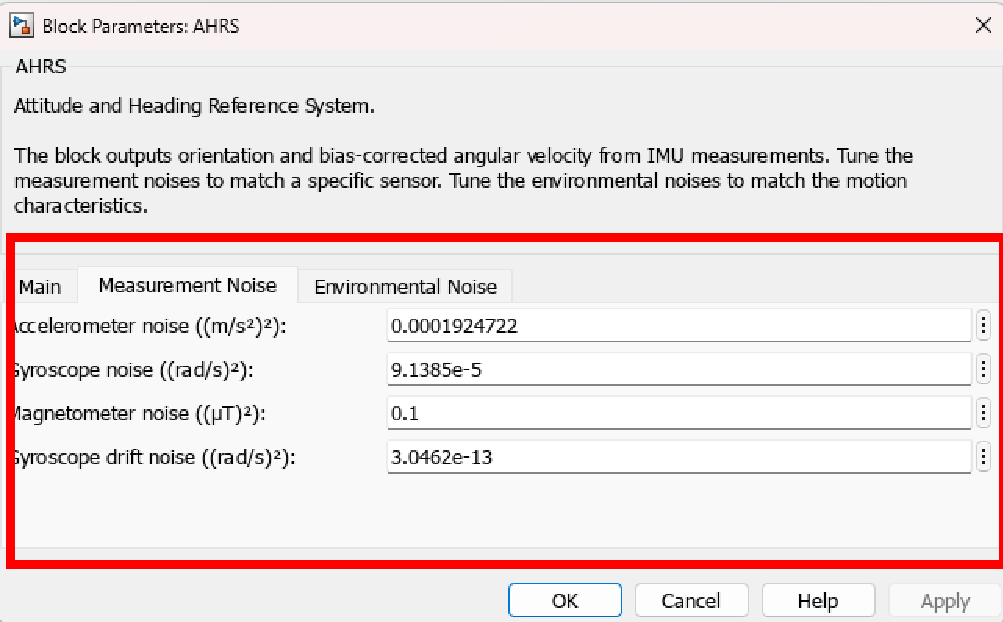
\includegraphics[width=\textwidth]{fig/Capitulo5/Caso_de_estudio_IMU/Generador_de_salidas/configuracion_AHRS_02.pdf}
        \caption{Configuración de parámetros 2}
        \label{fig:parametros_AHRS_02}
    \end{subfigure}
    \hfill
    % Cuarta imagen
    \begin{subfigure}[b]{0.45\textwidth}
        \centering
        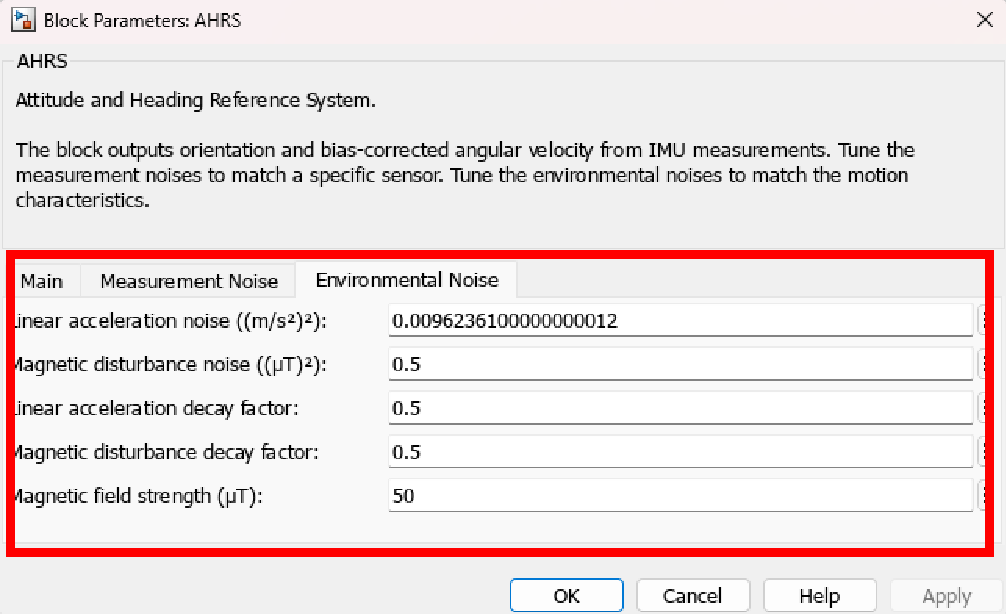
\includegraphics[width=\textwidth]{fig/Capitulo5/Caso_de_estudio_IMU/Generador_de_salidas/configuracion_AHRS_03.pdf}
        \caption{Configuración de parámetros 3}
        \label{fig:parametros_AHRS_03}
    \end{subfigure}

    \caption{Bloque para la simulación del comportamiento de la IMU}
    \label{fig:arreglo_AHRS}
\end{figure}

En la Figura \ref{fig:arreglo_AHRS}, se encontró el bloque denominado AHRS, este es un sistema que proporciona la estimación de la actitud y orientación de un objeto en 3D. Es por esto que se siguió una serie de configuraciones con el objetivo de lograr el correcto funcionamiento del módulo. Su principal función fue calcular la orientación del objeto usando datos de sensores como acelerómetros, giroscopios y magnetómetros. Por un lado en la Figura \ref{fig:lib_bloques_AHRS}, podemos observar el nombre del módulo en la Liberia de bloques. Una vez dentro de los parámetros de configuración del bloque tenemos en la Figura \ref{fig:parametros_AHRS_01}, los parámetros principales de configuración, seguido de esto en la Figura \ref{fig:parametros_AHRS_02}, tenemos los parámetros encargados del ruido de la medición. Finalmente en la Figura \ref{fig:parametros_AHRS_03} se configuran los parámetros relacionados con el ruido del ambiente. 
\newpage

\begin{figure}[htbp]
    \centering
    \begin{subfigure}[b]{0.35\textwidth}
        \centering
        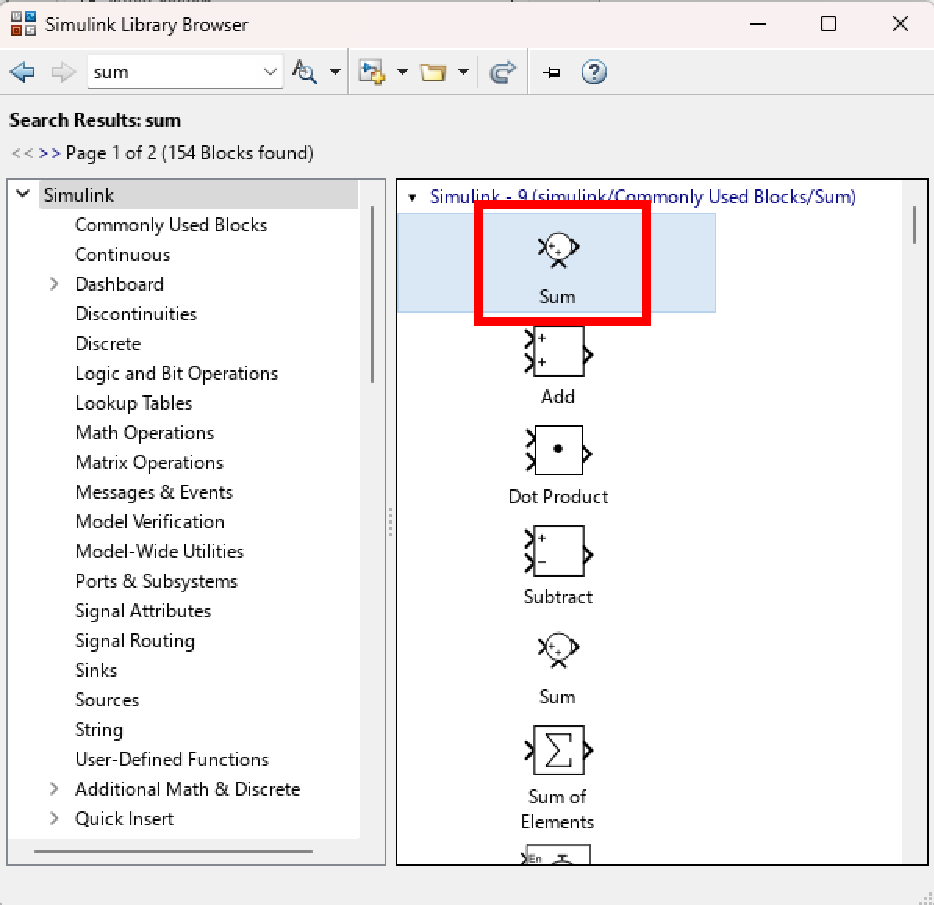
\includegraphics[width=\textwidth]{fig/Capitulo5/Caso_de_estudio_IMU/Generador_de_salidas/libreia_de_bloques_suma.pdf}
        \caption{Librería de bloques - Suma}
        \label{fig:lib_bloques_add_IMU}
    \end{subfigure}
    \hfill
    \begin{subfigure}[b]{0.45\textwidth}
        \centering
        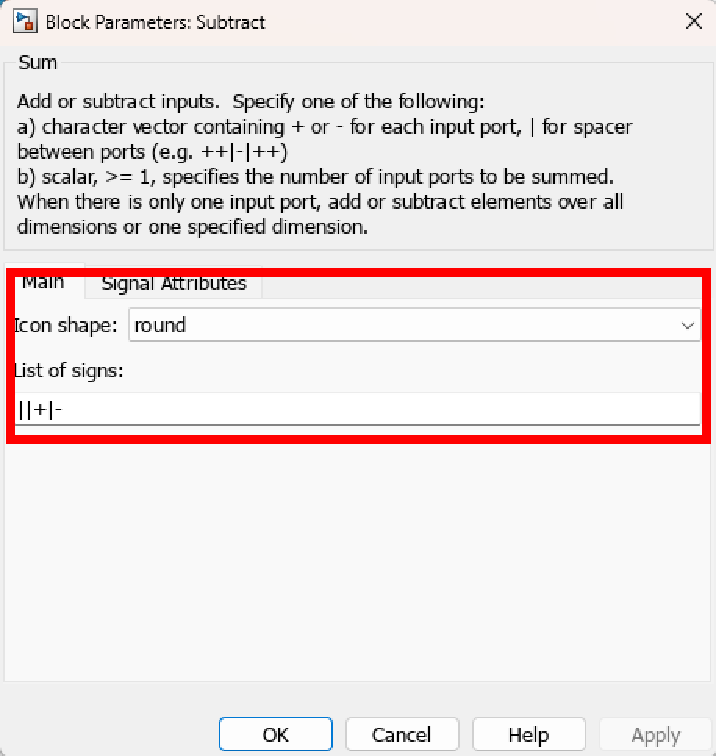
\includegraphics[width=\textwidth]{fig/Capitulo5/Caso_de_estudio_IMU/Generador_de_salidas/configuracion_bloque_suma.pdf}
        \caption{Configuración del bloque encargado de la suma de señales}
        \label{fig:config_add_IMU}
    \end{subfigure}
    \caption{Bloque para la suma de señales}
    \label{fig:add_of_some_signals}
\end{figure}

Para realizar una resta de señales se utilizó el bloque suma, el mismo se puede observar en la Figura \ref{fig:add_of_some_signals}. Se debe de realizar la diferencia para  calcular la desviación del giroscopio y de esta forma generar un archivo de salida con estos datos. 


\begin{figure}[htbp]
    \centering
    \begin{subfigure}[b]{0.35\textwidth}
        \centering
        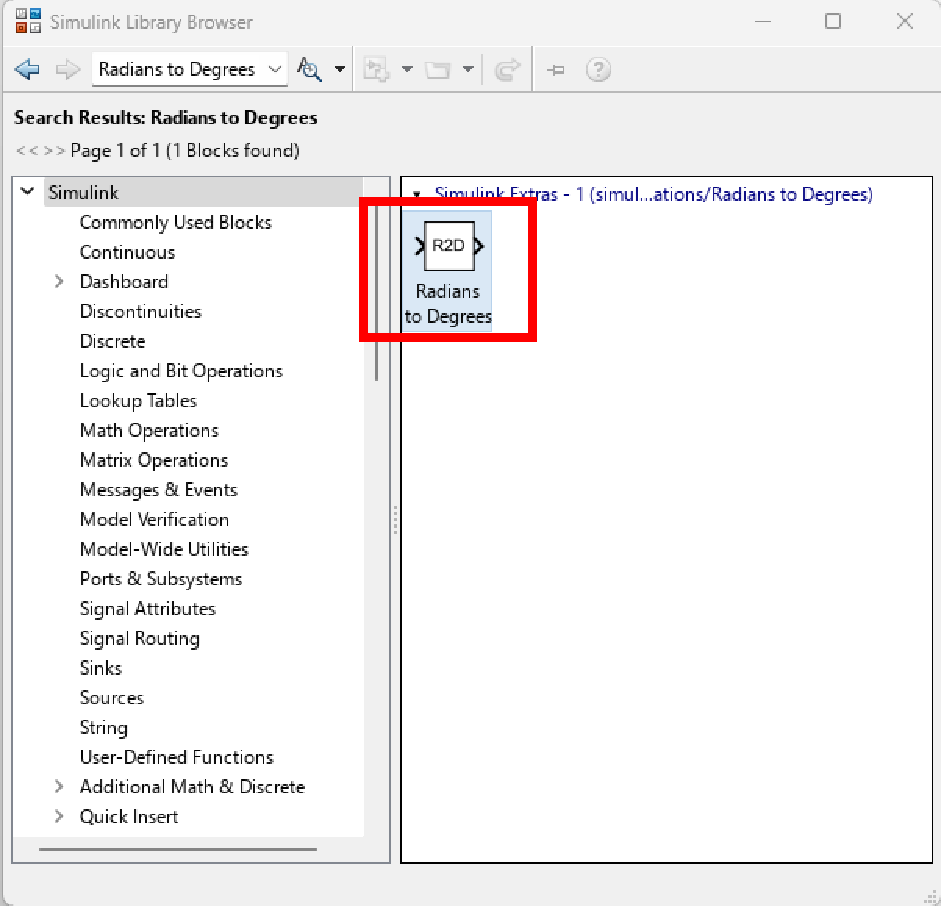
\includegraphics[width=\textwidth]{fig/Capitulo5/Caso_de_estudio_IMU/Generador_de_salidas/libreria_bloque__rad_2_deg.pdf}
        \caption{Librería de bloques - Conversor de radianes a grados}
        \label{fig:lib_bloques_R2D}
    \end{subfigure}
    \hfill
    \begin{subfigure}[b]{0.45\textwidth}
        \centering
        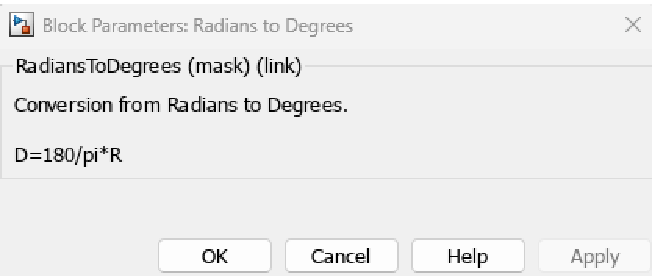
\includegraphics[width=\textwidth]{fig/Capitulo5/Caso_de_estudio_IMU//Generador_de_salidas/configuracion_rad_2_deg.pdf}
        \caption{Configuración del bloque conversor de radianes a grados}
        \label{fig:conf_bloques_R2D}
    \end{subfigure}
    \caption{Bloque para convertir de Radianes a grados}
    \label{fig:bloques_R2D}
\end{figure}

Los bloques de MATLAB trabajan utilizando las medidas de los ángulos en unidades de radianes, es por esto que se utilizó un bloque de transformación para  obtener los resultados en grados y que sean más sencillos de interpretar tanto en los datos de salida como en los gráficos elaborados.

\newpage

\begin{figure}[htbp]
    \centering
    \begin{subfigure}[b]{0.35\textwidth}
        \centering
        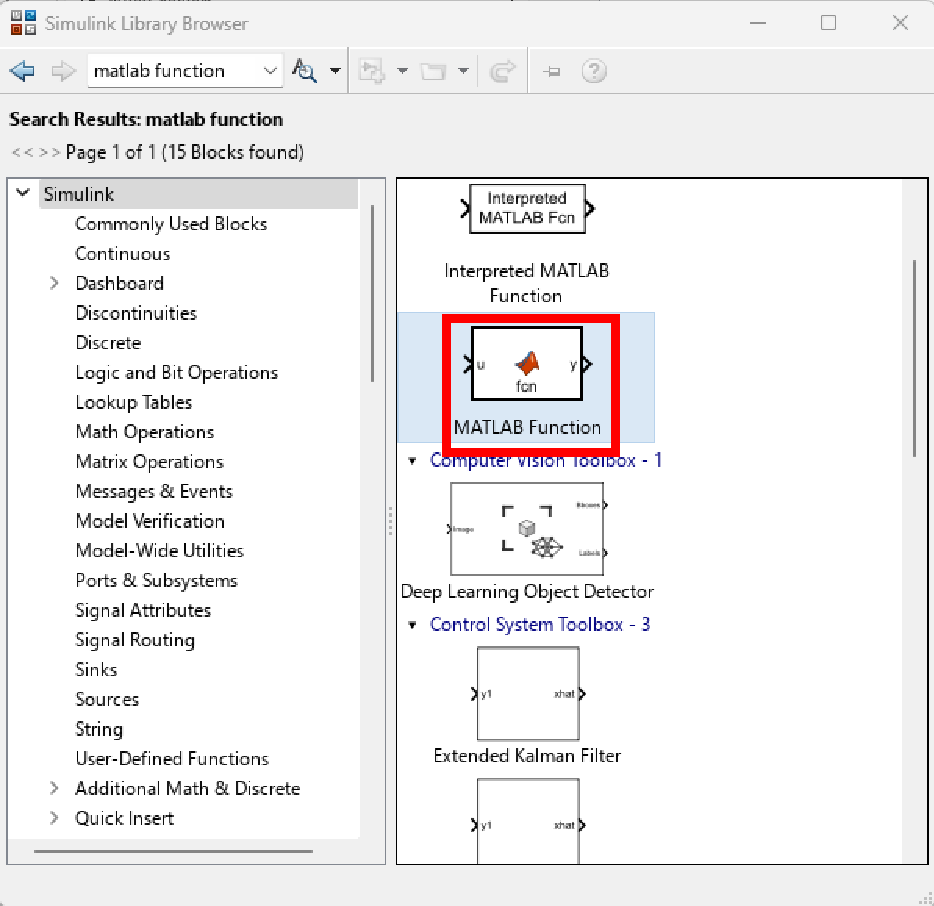
\includegraphics[width=\textwidth]{fig/Capitulo5/Caso_de_estudio_IMU/Generador_de_salidas/libreria_bloque_de_funcion.pdf}
        \caption{Librería de bloques - Función}
        \label{fig:lib_bloques_func}
    \end{subfigure}
    \hfill
    \begin{subfigure}[b]{0.45\textwidth}
        \centering
        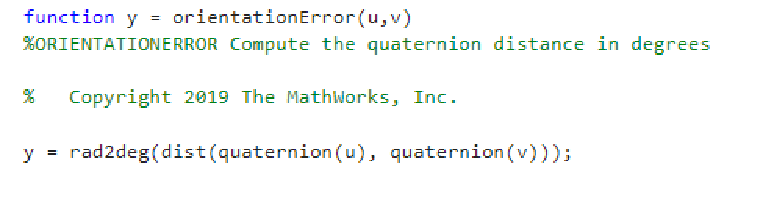
\includegraphics[width=\textwidth]{fig/Capitulo5/Caso_de_estudio_IMU/Generador_de_salidas/configuracion_codigo.pdf}
        \caption{Configuración del bloque de Función}
        \label{fig:config_bloques_func}
    \end{subfigure}
    \caption{Bloque para aplicar una función implementada mediante código}
    \label{fig:bloques_func}
\end{figure}

Finalmente se implementó un bloque de código encargado de calcular el error de orientación del sistema, esto con el fin de estimar la precisión con la cual el giroscopio simulado, en este caso de estudio se pudo determinar la orientación, en la Figura \ref{fig:lib_bloques_func} se observa el bloque en la librería, seguido de esto en la Figura \ref{fig:config_bloques_func} se observa el código implementado dentro de este bloque. El archivo se guardó bajo el nombre de (IMUFusionSimulinModel) y el tiempo de ejecución se estableció en 1000ms. 
\newpage

\subsection{Resultados de la simulación}\label{subsub:resultados_simulados_IMU}

\begin{figure}[htbp]
    \centering
    % Imagen superior
    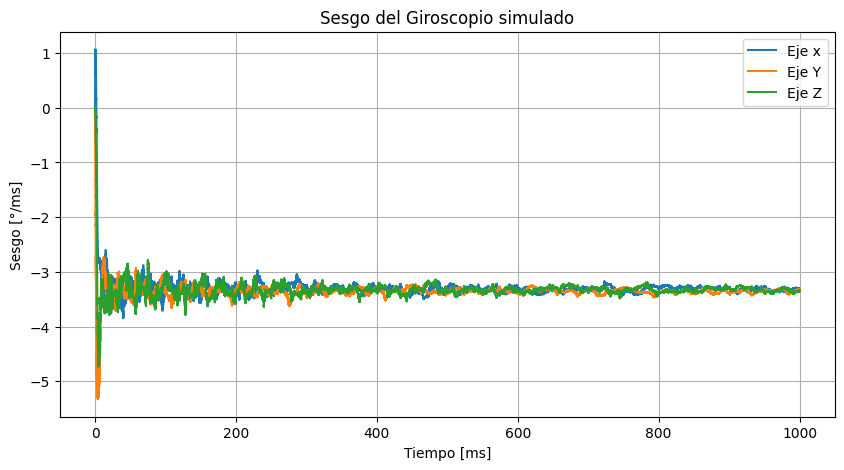
\includegraphics[scale=0.3]{fig/Capitulo5/Caso_de_estudio_IMU/data/simulated/sesgo_simulado.png}
    % Espacio entre las imágenes (opcional)
    \vspace{1cm}
    % Imagen inferior
    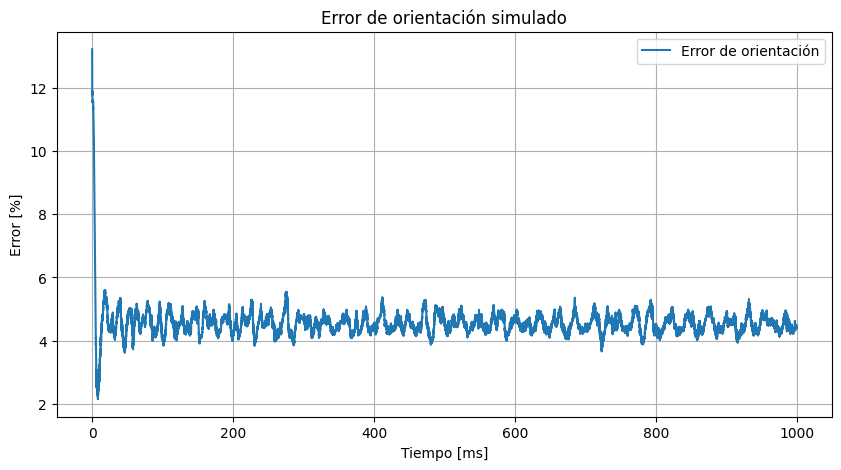
\includegraphics[scale=0.3]{fig/Capitulo5/Caso_de_estudio_IMU/data/simulated/error_de_orientacion_simulado.png}
    \caption{Datos simulados}
    \label{fig:data_simulated}
\end{figure}

Ejecutando el sistema en el entorno de simulación MATLAB Simulink se obtuvieron los resultados que se muestran en \ref{fig:data_simulated}, al lado izquierdo se observan los datos de la desviación simulada del sistema, mientras que, al lado derecho se observan los datos correspondientes a error de orientación. Cabe estacar que el resultado es esperado, ya que la diferencia entre la orientación estimada y la verdadera debería ser casi 4.7 [grados], que es la declinación en esta latitud y longitud y en el bloque IMU, al giroscopio se le dio una polarización de 0,0545 [rad/s] o 3,125 [grados/s], que debería coincidir con el valor de estado estacionario. En la siguiente sección se detallaron los pasos a seguir para la implementación de este sistema en la tarjeta de desarrollo por medio del flujo de trabajo desarrollado en el capítulo \ref{ch:especifico2}. 

\newpage

\subsection{Implementación en la Tarjeta de desarrollo mediante EmbedSynthGNC}


Para la implementación en la tarjeta de desarrollo ZedBoard se ejecutó el flujo de trabajo que se desarrolló en la sección \ref{sec:m2m_transformator}. El mismo es representado mediante el diagrama que se muestra en la Figura \ref{fig:m2m_matlab_simulink_coder}.

Primeramente se generaron los archivos de Código C desde MATLAB Simulink, para esto se deben de seguir el diagrama de la Figura \ref{fig:m2m_matlab_simulink_coder}. 

\begin{figure}[h!]
    \centering
    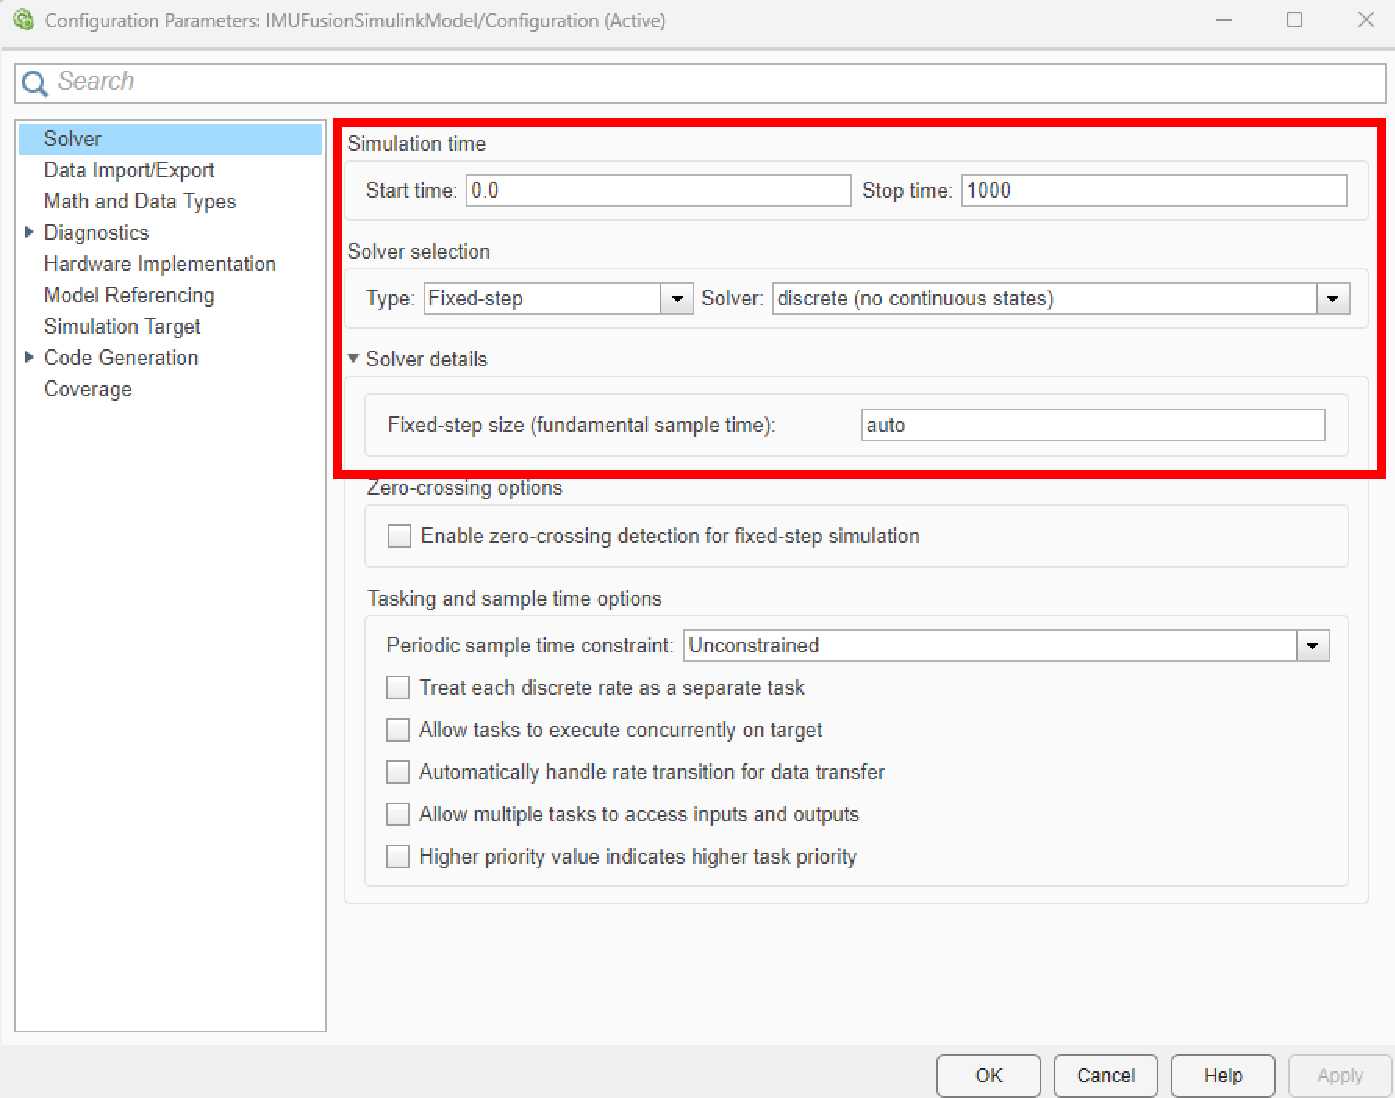
\includegraphics[width=0.5\textwidth]{fig/aditional/tiempo_ejecucion_imu.pdf}
    \caption{Definición del tiempo de ejecución del sistema}
    \label{fig:system_runtime_IMU}
\end{figure}

Como primer punto se realizaron las configuraciones que se muestran en la Figura \ref{fig:system_runtime_IMU} donde se definió el tiempo de ejecución del sistema, para este caso se estableció una ejecución de 1000 ms. 

\begin{figure}[h!]
    \centering
    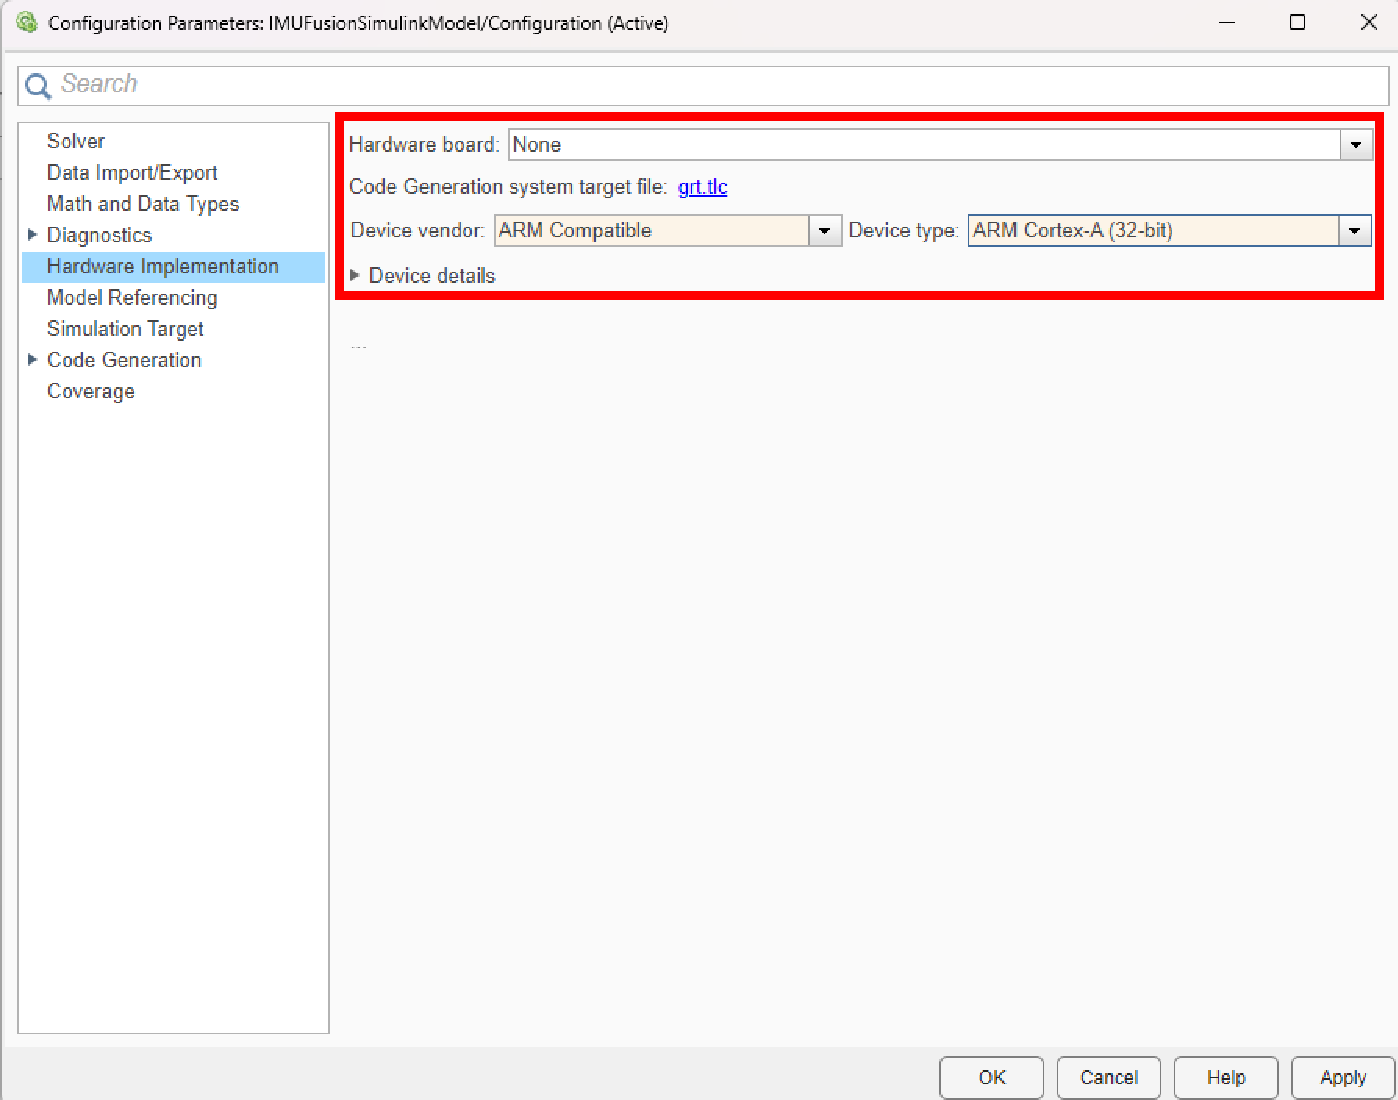
\includegraphics[width=0.5\textwidth]{fig/aditional/procesador_imu.pdf}
    \caption{Definición del procesador objetivo y arquitectura}
    \label{fig:system_target_IMU}
\end{figure}

Como se muestra en la Figura \ref{fig:system_target_IMU} se establecio el procesador objetivo y la arquitectura del mismo. Finalmente se definió el tipo de archivo de construcción el cual se puede observar en la Figura \ref{fig:pestana_config_output_file}. 

El archivo resultante fue un archivo llamado IMUFusionSimulinModel.zip seguido de esto se debe de  se exportaron los archivos al sistema Linux. Una vez exportados los archivos se descomprimieron los mismos en la carpeta denominada swap\_area.

\begin{figure}[h!]
    \centering
    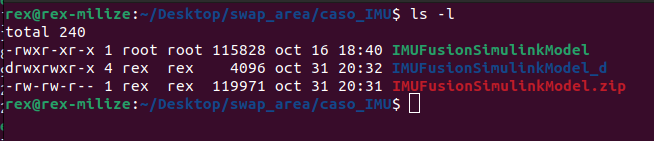
\includegraphics[width=0.5\textwidth]{fig/Capitulo5/Caso_de_estudio_IMU/retornos_consola/Screenshot from 2024-10-31 20-33-27.png}
    \caption{Archivo de construcción en el directorio swap\_area}
    \label{fig:swap_area_imu}
\end{figure}

\begin{lstlisting}[language=bash, caption={Compilacion del programa , Linux}, label=lst:build_cmake_file_IMU]
    cmake -DCMAKE_C_COMPILER=arm-linux-gnueabihf-gcc 
    CMakeLists.txt -DMATLAB_ROOT=/home/test/IMUFusionSimulinModel/R2024b/
\end{lstlisting}

Una vez fueron descomprimidos los archivos en el directorio denominado como swap\_area se enviaron al contenedor mediante el comando que se muestra en \ref{fig:swap_area_imu}. Luego se construyó el archivo responsable de la compilación del código C, esto se logro mediante el comando que se muestra en \ref{lst:build_cmake_file_IMU}. El archivo binario resultante se encuentra en la ruta /home/IMUFusionSimulinModel/IMURAW, este se envió al directorio denominado swap\_area, donde el mismo se exportó al contenedor encargado de integrarlo a la imagen generada mediante el marco de trabajo de Yocto y el flujo de trabajo de EmbedSynthGNC. 


Dentro del contendor del entorno Yocto se fue al directorio denominado meta-EmbedSynthGNC dentro del mismo se ingresó a la ruta (/poky/meta-EmbedsinthGNC/recipes-core) y en la misma se agrego un directorio con el nombre de (imu). Seguido, se inicializó el ambiente de trabajo mediante el uso del comando \ref{lst:yocto_ambient_set}. Una vez inicializado el ambiente de trabajo se agregó la nueva capa al archivo local.conf esto con el fin que el binario con el nombre IMUFusionSimulinModel sea incluido en la generación de la imagen. Finalmente se repitieron los pasos establecidos en \ref{sub:image2zedboard} donde se llevó a cabo la exportación de los archivos. Adicionalmente se preparó la memoria extraíble de la tarjeta de desarrollo para los nuevos archivos.

\newpage

\subsection{Resultados de la implementación}

\begin{figure}[htbp]
    \centering
    \begin{subfigure}[b]{0.35\textwidth}
        \centering
        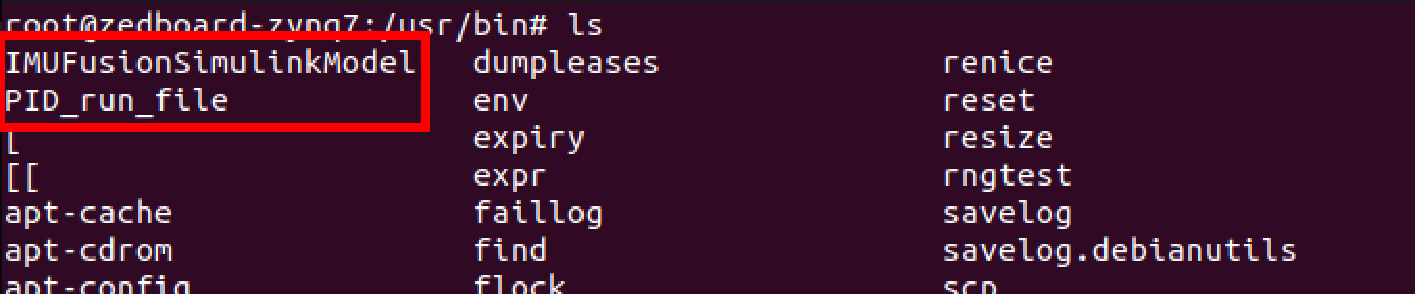
\includegraphics[width=\textwidth]{fig/aditional/consola_pid_imu.pdf}
        \caption{Tarjeta de desarrollo ZedBoard - IMU}
        \label{fig:imu_zedboard}
    \end{subfigure}
    \hfill
    \begin{subfigure}[b]{0.45\textwidth}
        \centering
        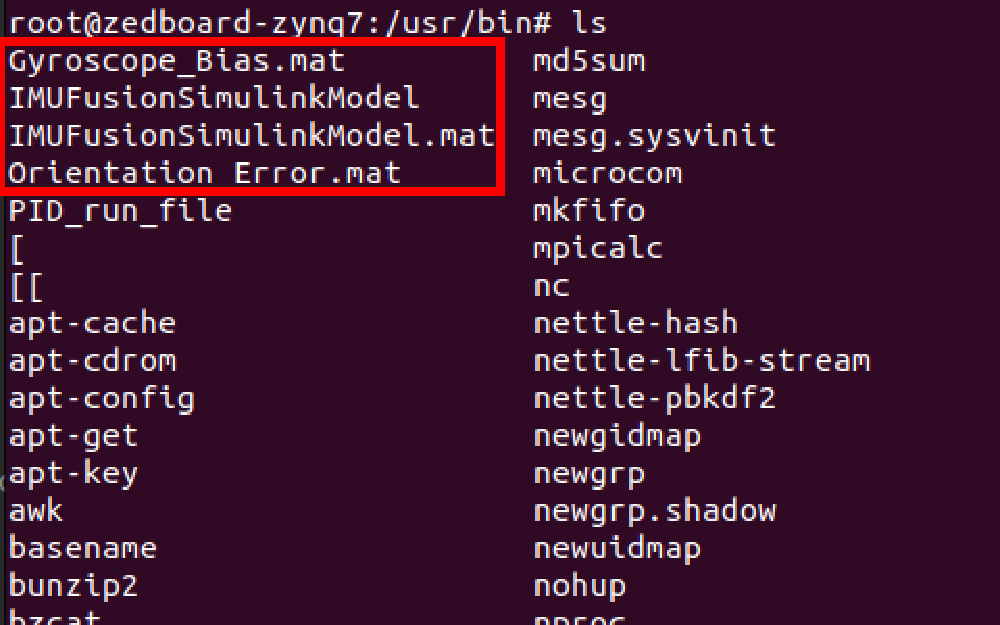
\includegraphics[width=\textwidth]{fig/aditional/consola_imu.pdf}
        \caption{Archivos de salida}
        \label{fig:out_files_IMU}
    \end{subfigure}
    \caption{Programa IMUFusionSimulinModel implementado en la tarjeta de desarrollo}
    \label{fig:IMU_ZEDBOARD}
\end{figure}
Como se puede observar en la Figura \ref{fig:imu_zedboard} se observa el binario contenido en la imagen dentro de la tarjeta de desarrollo. Una vez ejecutado el mismo se obtuvieron los archivos de salida que se muestran en la Figura \ref{fig:out_files_IMU}. 

\begin{figure}[htbp]
    \centering
    \begin{subfigure}[b]{0.35\textwidth}
        \centering
        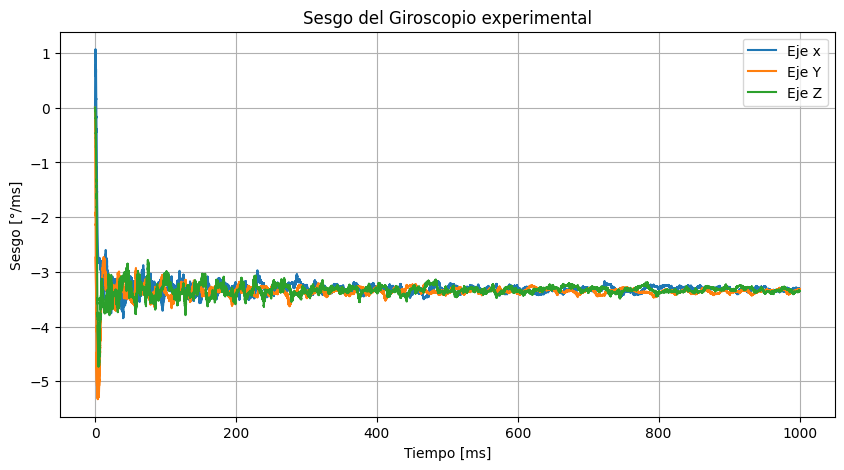
\includegraphics[width=\textwidth]{fig/Capitulo5/Caso_de_estudio_IMU/data/experimental/sesgo_experimental.png}
        \caption{Sesgo del giroscopio experimental}
        \label{fig:imu_sesgo_exp}
    \end{subfigure}
    \hfill
    \begin{subfigure}[b]{0.45\textwidth}
        \centering
        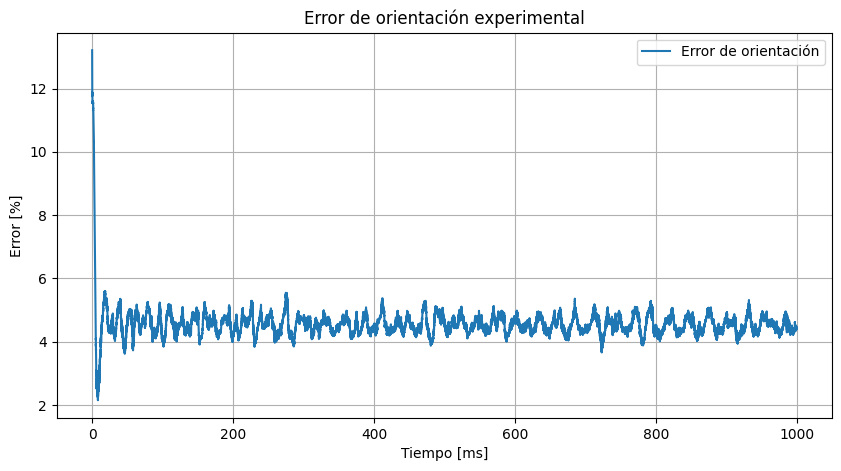
\includegraphics[width=\textwidth]{fig/Capitulo5/Caso_de_estudio_IMU/data/experimental/error_de_orientacion.png}
        \caption{Error de orientación experimental}
        \label{fig:out_files_IMU_eo_exp}
    \end{subfigure}
    \caption{Datos de archivo de salida IMU}
    \label{fig:IMU_ZEDBOARD_exp}
\end{figure}

Analizando los mismos mediante el programa de Python \ref{apx:comparacion_de_sennales_programa} se obtuvieron los gráficos que se muestran en \ref{fig:IMU_ZEDBOARD_exp}, donde en la Figura \ref{fig:imu_sesgo_exp} se muestra el gráfico relacionado con el sesgo del giroscopio en sus tres ejes de operación, y en la Figura \ref{fig:out_files_IMU_eo_exp} se muestra el gráfico de error de operación del giroscopio. Al realizar la comparación con los datos simulados \ref{subsub:resultados_simulados_IMU}, se obtuvieron los siguientes resultados para el análisis de error.

\begin{table}[htbp!]
    \centering
    \caption{Precisión de la implementación del caso de estudio IMU respecto al eje X}
    \label{tab:filter-errorz}
    \begin{tabular}{ll}
    Métrica                       & Error \\ \hline
    Error promedio absoluto         &   $2.31 \times 10^{-15}$ [grados/s]    \\
    Error cuadrático medio          &   $3.09 \times 10^{-15}$ $[grados/s^{2}]$    \\
    Raíz del error cuadrático medio &   $9.56 \times 10{-30}$ [grados/s]  
    \end{tabular}
    \end{table}


\begin{table}[htbp!]
    \centering
    \caption{Precisión de la implementación del caso de estudio IMU respecto al eje Y}
    \label{tab:filter-errory}
    \begin{tabular}{ll}
    Métrica                       & Error \\ \hline
    Error promedio absoluto         &   $2.36 \times 10^{-15}$ [grados/s]    \\
    Error cuadrático medio          &   $3.29 \times 10^{-15}$ $[grados/s^{2}]$    \\
    Raíz del error cuadrático medio &   $1.08 \times 10{-29}$ [grados/s]  
    \end{tabular}
    \end{table}

\begin{table}[htbp!]
    \centering
    \caption{Precisión de la implementación del caso de estudio IMU respecto al eje Z}
    \label{tab:filter-errorz}
    \begin{tabular}{ll}
    Métrica                       & Error \\ \hline
    Error promedio absoluto         &   $3.19 \times 10^{-15}$ [grados/s]    \\
    Error cuadrático medio          &   $4.58 \times 10^{-15}$ $[grados/s^{2}]$    \\
    Raíz del error cuadrático medio &   $2.10 \times 10{-29}$ [grados/s]  
    \end{tabular}
    \end{table}

De los cuales se puede determinar que dado el orden de magnitud tan pequeño de los errores en cada eje, las mediciones del giroscopio son altamente precisas, con variaciones mínimas. Las diferencias entre los ejes (ligeramente más altas en el eje Z) podrían deberse a factores menores de calibración o sensibilidad en el giroscopio, pero en general se logra obtener un desempeño excelente.


Por otro lado los datos relacionados con el error de orientación se obtiene que las diferencias mostradas en estas gráficas es dé.

\begin{table}[htbp!]
    \centering
    \caption{Precisión de la implementación del caso de estudio IMU respecto error de orientación compuesto}
    \label{tab:filter-errorzgrad}
    \begin{tabular}{ll}
    Métrica                       & Error \\ \hline
    Error promedio absoluto         &   $1.28 \times 10^{-13}$ [grados]\\
    Error cuadrático medio          &   $2.12 \times 10^{-13}$ $[grados^{2}]$    \\
    Raíz del error cuadrático medio &   $4.51 \times 10{-26}$ [grados]  
    \end{tabular}
    \end{table}


Aunque el error en la orientación es de una magnitud algo mayor que en los ejes individuales del giroscopio, sigue siendo muy pequeño. Esto sugiere que el sistema de orientación es preciso, aunque hay un margen de acumulación de error que sería esperado en cálculos de orientación que integran múltiples ejes. 

\newpage

\section{Caso de estudio 3 - PID}

Finalmente como último caso de estudio se desarrolló un controlador PID (Proporcional-Integral-Derivativo) es una herramienta clave en los sistemas de control automático, diseñada para minimizar el error entre una señal de referencia y la señal de salida real. Su importancia radica en su capacidad para ajustar la respuesta del sistema, logrando un equilibrio entre rapidez y estabilidad. Esto permite que el controlador maneje eficazmente perturbaciones y cambios en el entorno, siendo aplicable a una variedad de sistemas, como motores eléctricos, sistemas de calefacción y procesos industriales complejos.

En el contexto de MATLAB y Simulink, estas herramientas ofrecen una plataforma visual que facilita la implementación y ajuste de controladores PID. A través de bloques específicos en Simulink, los ingenieros pueden modificar en tiempo real los parámetros proporcional, integral y derivativo, observando directamente cómo estos ajustes afectan la salida del sistema. Esta capacidad de simulación y diseño iterativo no solo optimiza el rendimiento del sistema controlado, sino que también proporciona un entorno propicio para la experimentación y el aprendizaje práctico en el campo del control automático.


\subsection{Implementación en MATLAB Simulink}

\begin{figure}[h!]
    \centering
    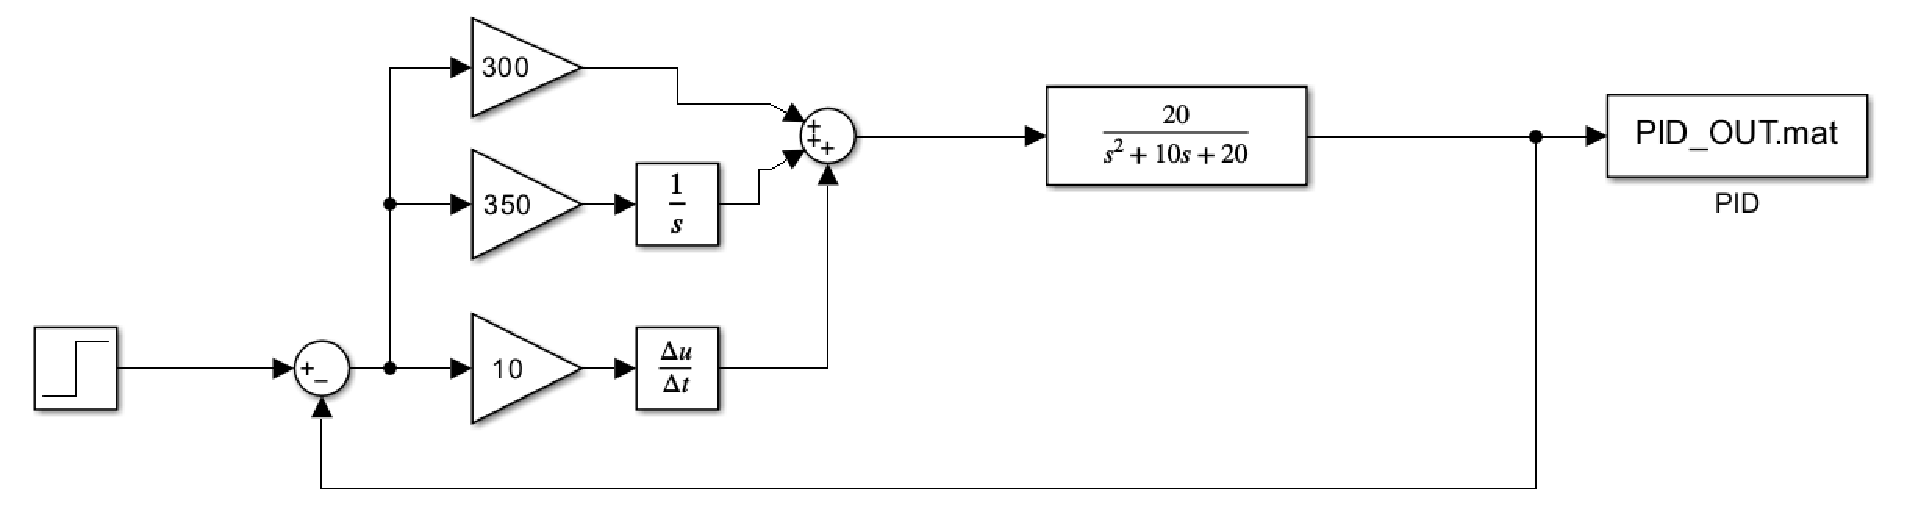
\includegraphics[width=0.8\textwidth]{fig/Capitulo5/Caso_de_estudio_PID/PID_Diagram.pdf}
    \caption{Diagrama completo del caso de estudio 3 - PID }
    \label{fig:caso_de_estudio_3_PID}
\end{figure}


Como se observa en la Figura \ref{fig:caso_de_estudio_3_PID}, este es el caso de estudio que se propuso en \cite{microcontrollerslab_pid_controller_design}, a este caso de estudio se le realizaron unas modificaciones de acuerdo al funcionamiento deseado, siempre generando datos en el ámbito de simulación en MATLAB para luego contrastar los mismos con los datos obtenidos en la ejecución del modelo en la tarjeta de desarrollo seleccionada.

\subsection{Bloques utilizados para la implementación}

Los bloques utilizados se obtuvieron en la librería de bloques de MATLAB Simulink. A continuación se muestran los bloques empleados, así como la configuración de los mismos para la correcta operación del modelo.

%%step
\begin{figure}[htbp]
    \centering
    \begin{subfigure}[b]{0.35\textwidth}
        \centering
        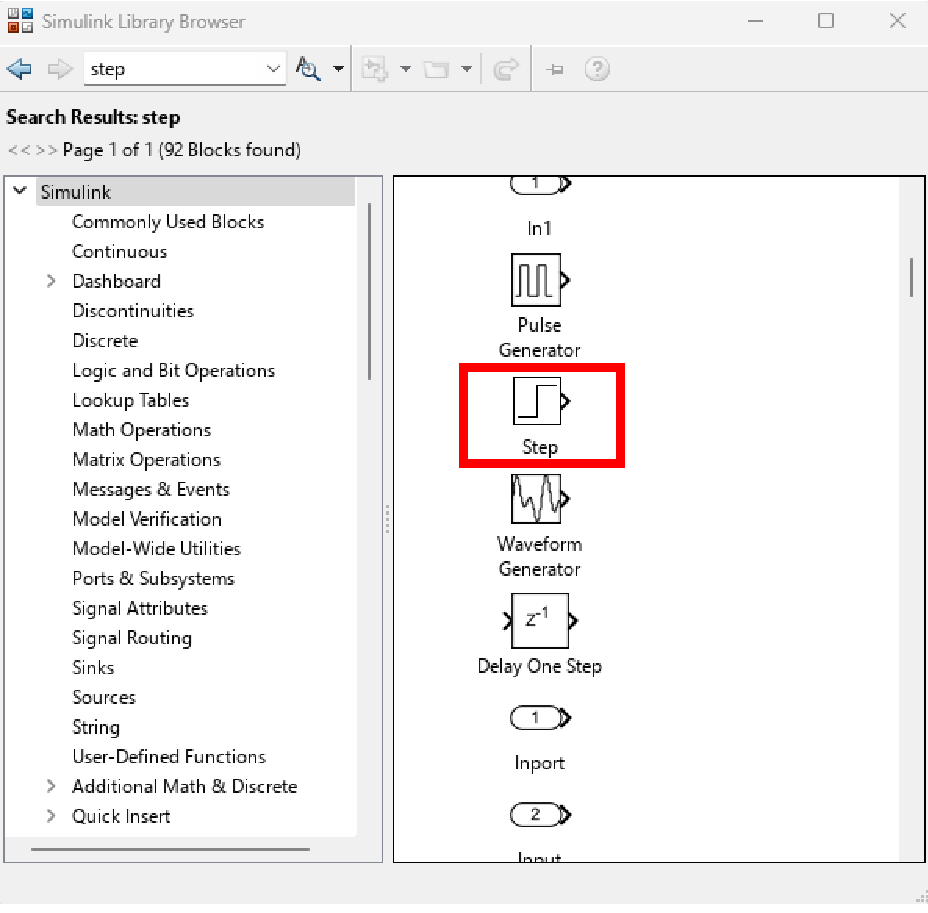
\includegraphics[width=\textwidth]{fig/Capitulo5/Caso_de_estudio_PID/lib_step.pdf}
        \caption{Librería de bloques - Escalon}
        \label{fig:step_lib}
    \end{subfigure}
    \hfill
    \begin{subfigure}[b]{0.45\textwidth}
        \centering
        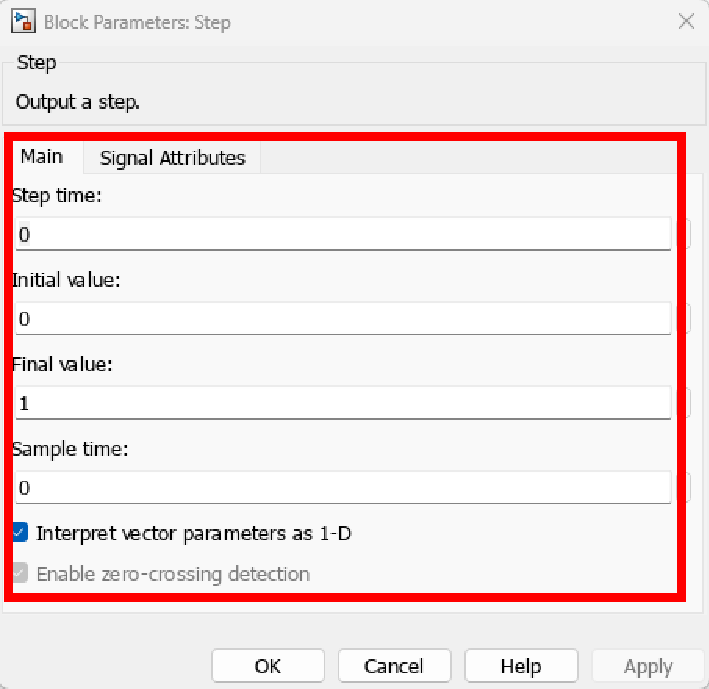
\includegraphics[width=\textwidth]{fig/Capitulo5/Caso_de_estudio_PID/config_step.pdf}
        \caption{Configuración del bloque encargado de generar un escalon }
        \label{fig:step_conf}
    \end{subfigure}
    \caption{Bloque escalon}
    \label{fig:step_block}
\end{figure}
\newpage

Primeramente para la implementación del modelo que se muestra en la Figura \ref{fig:caso_de_estudio_3_PID}, se utilizó el bloque que se muestra en la Figura \ref{fig:step_block}, el mismo se puedo encontrar en la librería de bloques como se muestra en la Figura \ref{fig:step_lib}, además de esto la configuración del mismo se observa en la Figura \ref{fig:step_conf}.

%%integrator
\begin{figure}[htbp]
    \centering
    \begin{subfigure}[b]{0.35\textwidth}
        \centering
        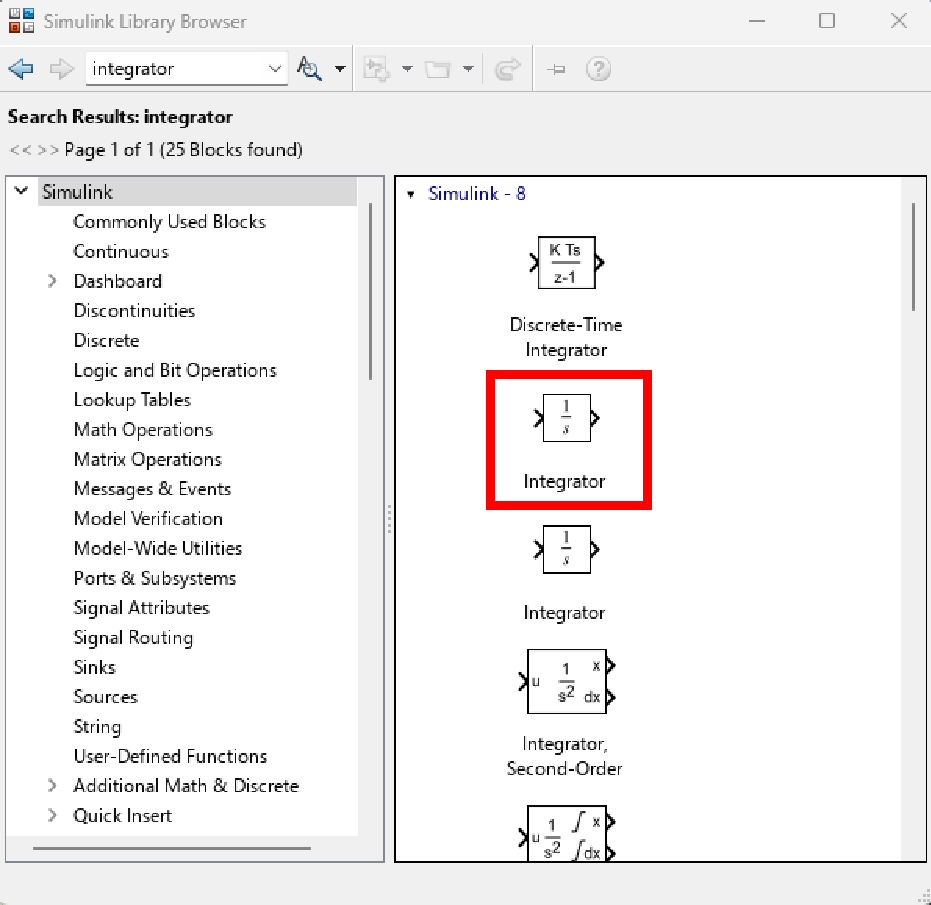
\includegraphics[width=\textwidth]{fig/Capitulo5/Caso_de_estudio_PID/lib_integrator.pdf}
        \caption{Librería de bloques - Integrador}
        \label{fig:int_PID_lib}
    \end{subfigure}
    \hfill
    \begin{subfigure}[b]{0.45\textwidth}
        \centering
        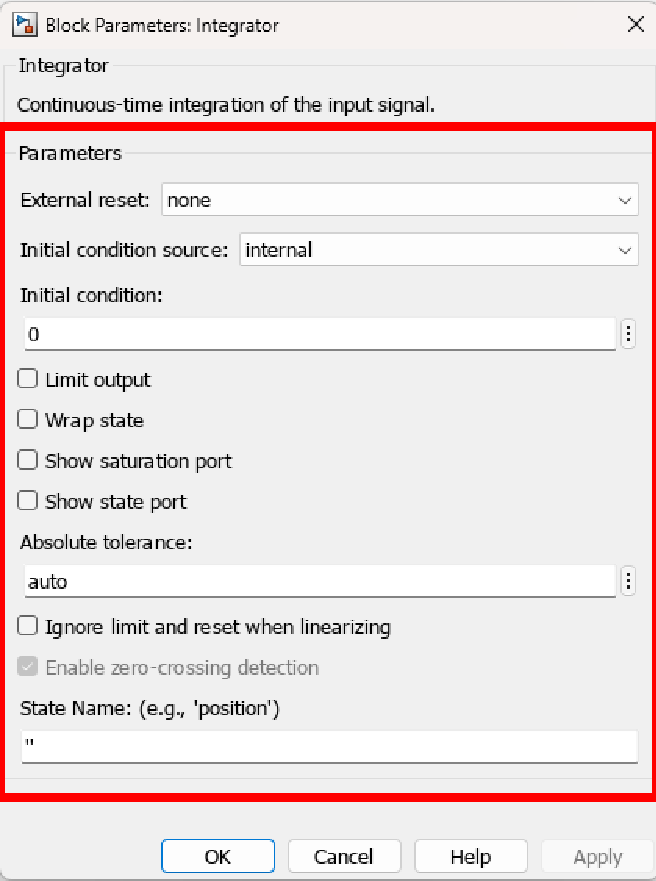
\includegraphics[width=\textwidth]{fig/Capitulo5/Caso_de_estudio_PID/config_integrator.pdf}
        \caption{Configuración del bloque encargado de Integrar}
        \label{fig:int_conf_PID}
    \end{subfigure}
    \caption{Bloque integrador}
    \label{fig:int_block}
\end{figure}

Por un lado, al realizar la implementación del controlador PID por separado se utilizó un bloque especializado para la integración, este se muestra en la Figura \ref{fig:int_block}, es obtenido en la librería de bloques como se muestra en la Figura \ref{fig:int_PID_lib}. La configuración de este bloque se observa en la Figura \ref{fig:int_conf_PID}.

\newpage

%%derivative
\begin{figure}[htbp]
    \centering
    \begin{subfigure}[b]{0.35\textwidth}
        \centering
        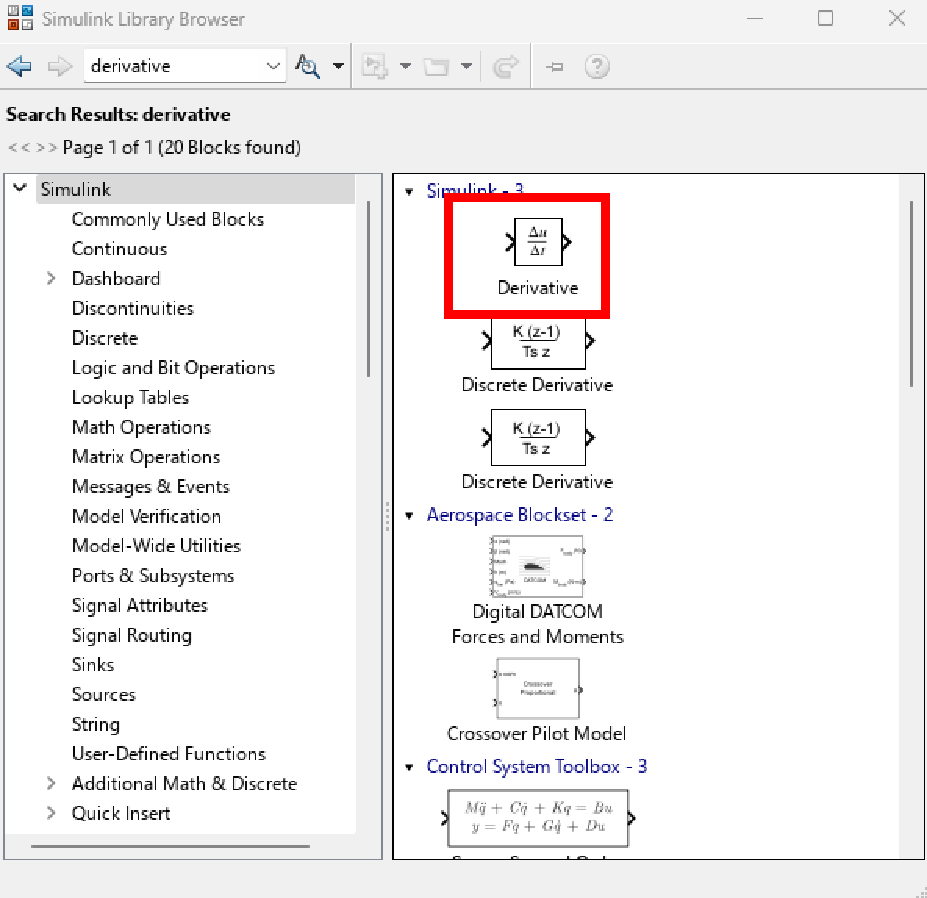
\includegraphics[width=\textwidth]{fig/Capitulo5/Caso_de_estudio_PID/lib_derivative.pdf}
        \caption{Librería de bloques - Derivador}
        \label{fig:dev_PID_lib}
    \end{subfigure}
    \hfill
    \begin{subfigure}[b]{0.45\textwidth}
        \centering
        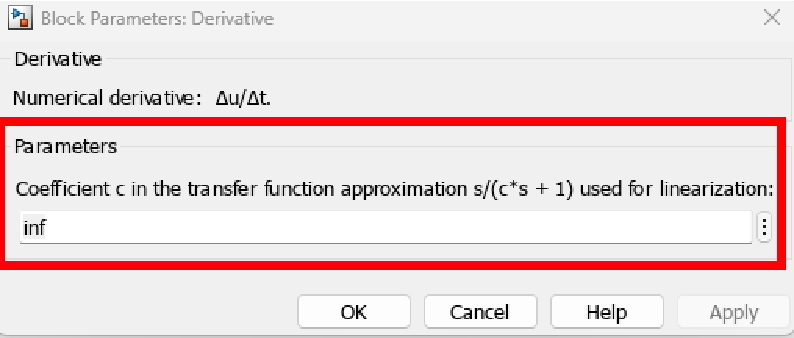
\includegraphics[width=\textwidth]{fig/Capitulo5/Caso_de_estudio_PID/config_derivative.pdf}
        \caption{Configuración del bloque encargado de derivar}
        \label{fig:dev_PID_conf}
    \end{subfigure}
    \caption{Bloque derivador}
    \label{fig:dev_block}
\end{figure}

Por otro lado, tenemos un bloque especializado para la derivación, se logro mediante el uso del bloque de la Figura \ref{fig:dev_block}, el mismo se obtuvo de la librería de bloques como se muestra en la Figura \ref{fig:dev_PID_lib}. La configuración de este bloque se observa en la Figura \ref{fig:dev_conf_PID}. 

%%
\begin{figure}[htbp]
    \centering
    \begin{subfigure}[b]{0.35\textwidth}
        \centering
        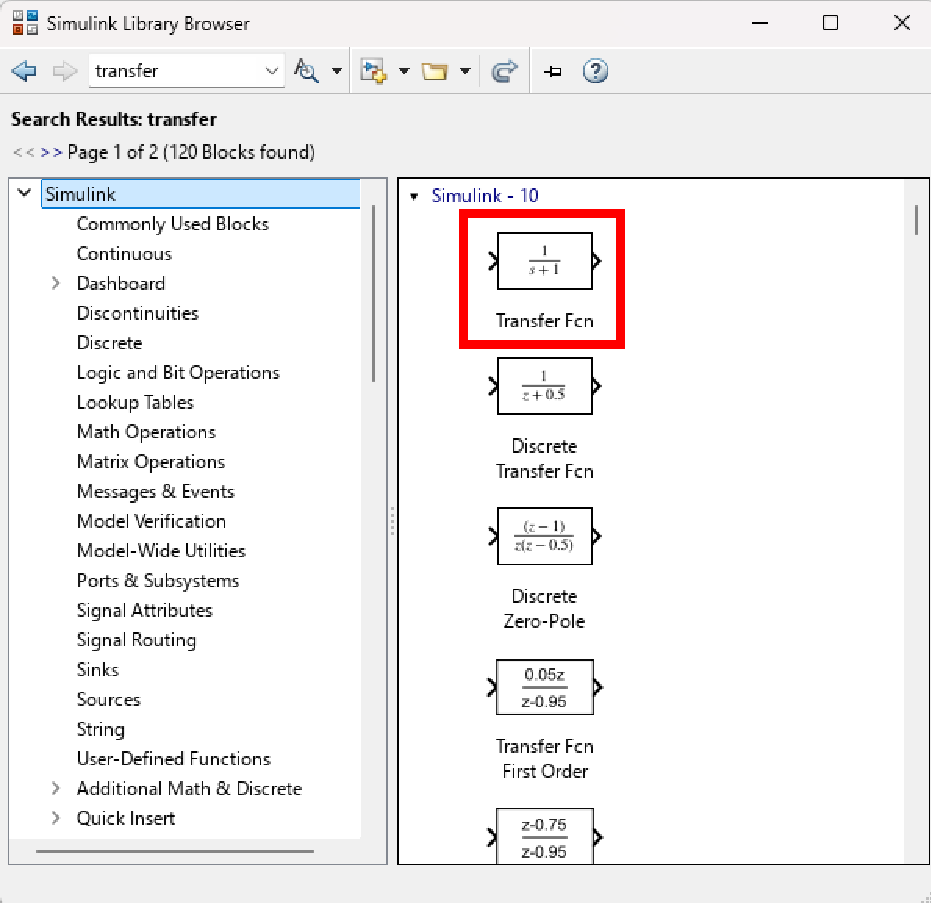
\includegraphics[width=\textwidth]{fig/Capitulo5/Caso_de_estudio_PID/Transfer_func.pdf}
        \caption{Librería de bloques - Funcion de trasnferencia}
        \label{fig:tf_func_lib}
    \end{subfigure}
    \hfill
    \begin{subfigure}[b]{0.45\textwidth}
        \centering
        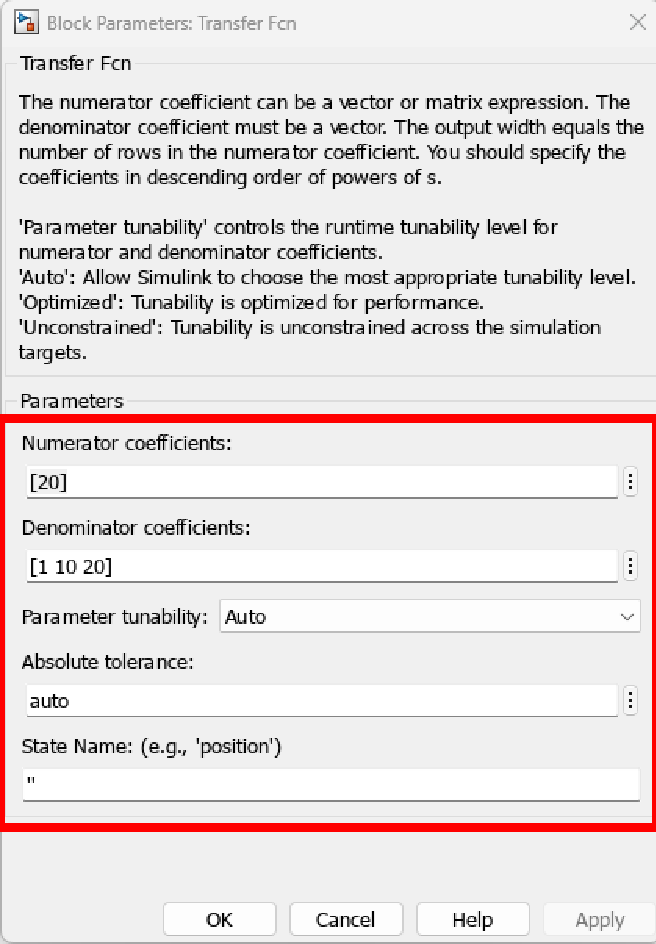
\includegraphics[width=\textwidth]{fig/Capitulo5/Caso_de_estudio_PID/config_transfer_function.pdf}
        \caption{Configuración del bloque encargado de aplicar la funcion de transferencia}
        \label{fig:tf_func_conf}
    \end{subfigure}
    \caption{Bloque funcion de transferencia}
    \label{fig:tf_func_block}
\end{figure}

Al tratarse de la implementación de un control PID el mismo contó con la función de transferencia, esta fue implementada mediante el bloque que de la Figura \ref{fig:tf_func_block}, el mismo se encontró en la librería de bloques como se observa en la Figura \ref{fig:tf_func_lib}, además de esto la configuración de la función de transferencia se observa en la Figura \ref{fig:tf_func_conf}.

%%gain
\begin{figure}[htbp]
    \centering
    % Primera imagen
    \begin{subfigure}[b]{0.35\textwidth}
        \centering
        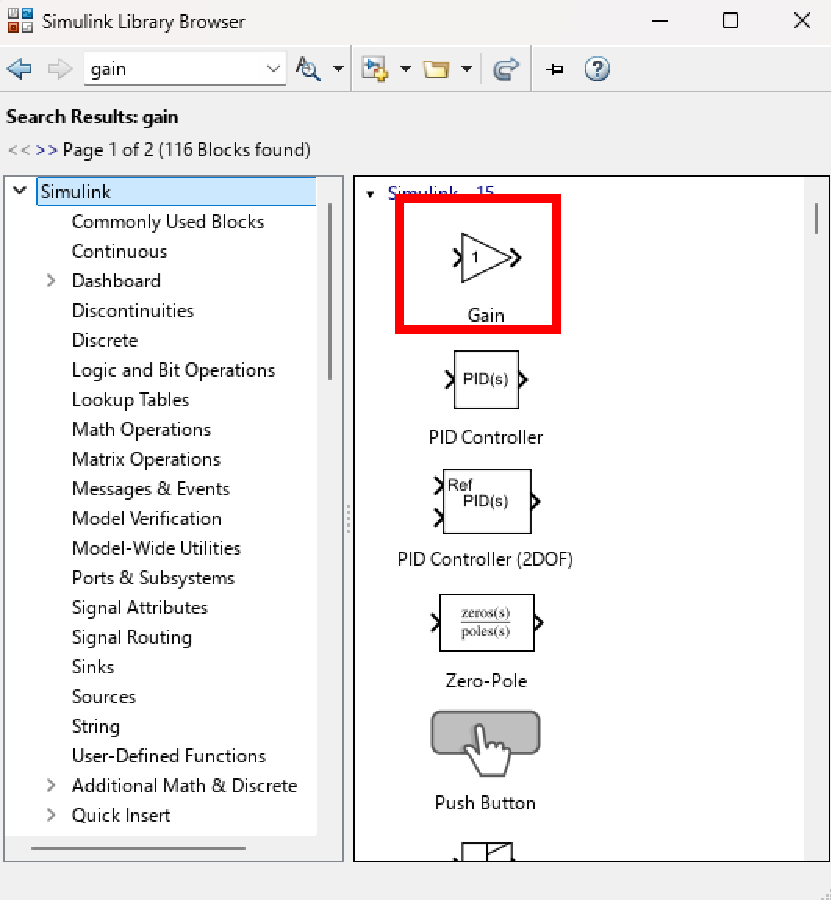
\includegraphics[width=\textwidth]{fig/Capitulo5/Caso_de_estudio_PID/lib_gain.pdf}
        \caption{Librería de bloques - Ganancia}
        \label{fig:lib_bloques_gain}
    \end{subfigure}
    \hfill
    % Segunda imagen
    \begin{subfigure}[b]{0.45\textwidth}
        \centering
        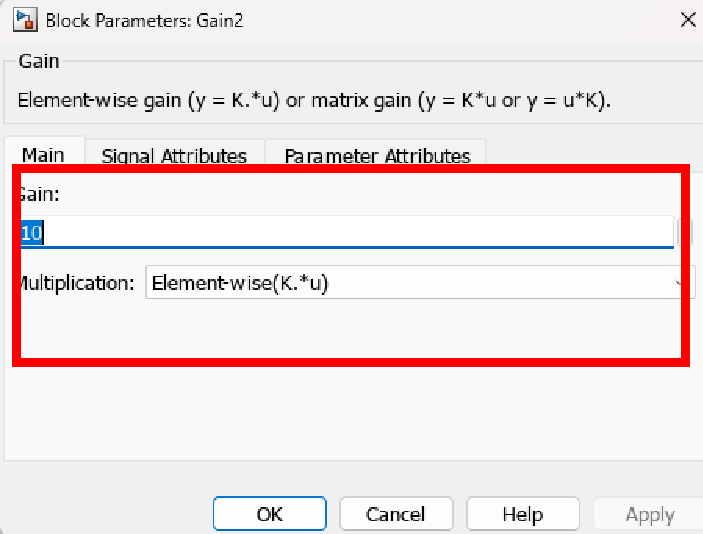
\includegraphics[width=\textwidth]{fig/Capitulo5/Caso_de_estudio_PID/config_gain_10.pdf}
        \caption{Configuración de parámetros 1}
        \label{fig:parametros_gain_01}
    \end{subfigure}
    \hfill
    % Tercera imagen
    \begin{subfigure}[b]{0.45\textwidth}
        \centering
        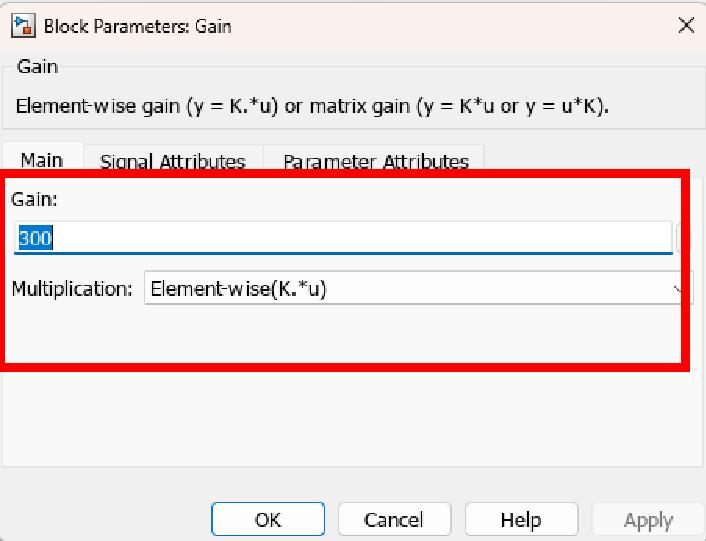
\includegraphics[width=\textwidth]{fig/Capitulo5/Caso_de_estudio_PID/config_gain_300.pdf}
        \caption{Configuración de parámetros 2}
        \label{fig:parametros_gain_02}
    \end{subfigure}
    \hfill
    % Cuarta imagen
    \begin{subfigure}[b]{0.45\textwidth}
        \centering
        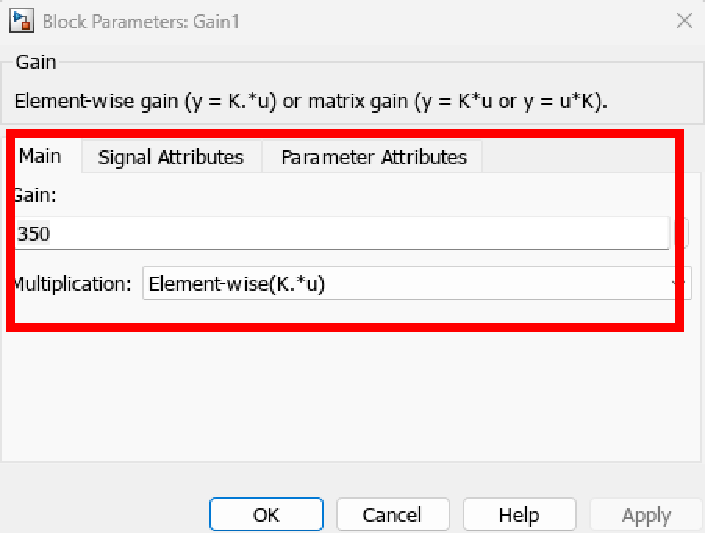
\includegraphics[width=\textwidth]{fig/Capitulo5/Caso_de_estudio_PID/config_gain_350.pdf}
        \caption{Configuración de parámetros 3}
        \label{fig:parametros_gain_03}
    \end{subfigure}

    \caption{Bloque para la asignación de ganancias}
    \label{fig:arreglo_gain}
\end{figure}

También, se ingresaron los valores de las ganancias esto se realiza por medio del bloque de la Figura \ref{fig:arreglo_gain}, se logró mediante la implementación de tres bloques de ganancia el primero se generó con la configuración que se muestra en la Figura \ref{fig:parametros_gain_01}, el segundo se estableció según los parámetros indicados en la Figura \ref{fig:parametros_gain_02} y finalmente el tercero se configuró como lo indica la Figura \ref{fig:parametros_gain_03}. 

%%add
\begin{figure}[htbp]
    \centering
    % Primera imagen
    \begin{subfigure}[b]{0.35\textwidth}
        \centering
        \includegraphics[width=\textwidth]{fig/Capitulo5/Caso_de_estudio_PID/lib_suma.pdf}
        \caption{Librería de bloques - suma}
        \label{fig:lib_bloques_add}
    \end{subfigure}
    \hfill
    % Segunda imagen
    \begin{subfigure}[b]{0.45\textwidth}
        \centering
        \includegraphics[width=\textwidth]{fig/Capitulo5/Caso_de_estudio_PID/config_sum_02.pdf}
        \caption{Configuración de parámetros 1}
        \label{fig:parametros_add_01}
    \end{subfigure}
    \hfill
    % Tercera imagen
    \begin{subfigure}[b]{0.45\textwidth}
        \centering
        \includegraphics[width=\textwidth]{fig/Capitulo5/Caso_de_estudio_PID/config_sum_01.pdf}
        \caption{Configuración de parámetros 2}
        \label{fig:parametros_add_02}
    \end{subfigure}

    \caption{Bloques encargados de sumas}
    \label{fig:arreglo_add}
\end{figure}

\newpage

Finalmente se implementaron dos bloques de suma, el primer bloque se encargo de realizar la realimentación del sistema de control, el mismo se implementa haciendo uso de bloque de la librería que se observa en la Figura \ref{fig:lib_bloques_add}, esto mediante el uso de la configuración establecida en la Figura \ref{fig:parametros_add_01}, por otro lado el segundo bloque de suma se encargo de sumar las tres señales de salida del controlador PID este bloque se configuró como se muestra en la Figura \ref{fig:parametros_add_02}. Una vez implementado el sistema el archivo se guardó bajo el nombre de (PIDRunFile) y el tiempo de ejecución se debe se estableció para 0.5ms. 

\subsection{Resultados simulados}\label{subsub:resultados_simulados_PID}

\begin{figure}[h!]
    \centering
    \includegraphics[width=0.8\textwidth]{fig/Capitulo5/Caso_de_estudio_PID/datos/simulada.png}
    \caption{Salida simulada - PID }
    \label{fig:salida_simulada_PID}
\end{figure}


Cuando se ejecutó el sistema en el entorno de simulación MATLAB Simulink se obtuvieron los resultados que se muestran en \ref{fig:salida_simulada_PID}. Cabe estacar que el resultado es esperado, ya que el valor de estado estacionario esperado para este modelo debería ser de 1.02 V. En las próximas secciones se detallaron los pasos a seguir para la implementación de este sistema en la tarjeta de desarrollo por medio del flujo de trabajo que se desarrolló en capítulo \ref{ch:especifico2}. 


\subsection{Implementación en la Tarjeta de desarrollo mediante EmbedSynthGNC}

Para la implementación en la tarjeta de desarrollo ZedBoard se ejecutó el flujo de trabajo que se muestra en la sección \ref{sec:m2m_transformator}. El mismo es representado mediante el diagrama que se muestra en la Figura \ref{fig:m2m_matlab_simulink_coder}.

Primeramente se generaron los archivos de Código C desde MATLAB Simulink, para esto se siguió el diagrama de la Figura \ref{fig:m2m_matlab_simulink_coder}. 

\begin{figure}[h!]
    \centering
    \includegraphics[width=0.5\textwidth]{fig/aditional/procesador_pid.pdf}
    \caption{Definición del procesador objetivo y arquitectura}
    \label{fig:system_target_PID}
\end{figure}

Como se muestra en la Figura \ref{fig:system_target_PID} se estableció el procesador objetivo y la arquitectura del mismo. Finalmente se definió el tipo de archivo de construcción el cual se observa en la Figura \ref{fig:pestana_config_output_file}. 

El archivo resultante fue un archivo llamado PIDRunFile.zip seguido de esto se exportaron los archivos al sistema Linux. Una vez exportados los archivos se descomprimieron los mismos en la carpeta denominada swap\_area.

\begin{figure}[h!]
    \centering
    \includegraphics[width=0.5\textwidth]{fig/Capitulo5/Caso_de_estudio_PID/retornos_consola/Screenshot from 2024-10-31 20-21-37.png}
    \caption{Archivo de construcción en el directorio swap area}
    \label{fig:swap_area_PID}
\end{figure}


\begin{lstlisting}[language=bash, caption={Compilacion del programa , Linux}, label=lst:build_cmake_file_PID]
    cmake -DCMAKE_C_COMPILER=arm-linux-gnueabihf-gcc 
    CMakeLists.txt -DMATLAB_ROOT=/home/test/PIDRunFile/R2024b/
\end{lstlisting}

Una vez descomprimidos los archivos en el directorio denominado como swap\_area se enviaron al contenedor mediante el comando que se muestra en \ref{fig:swap_area_PID}. Una vez dentro del contenedor se construyó el archivo responsable de la compilación del código C, esto se logro mediante el comando que se muestra en \ref{lst:build_cmake_file_PID}. El archivo binario resultante se encuentra en la ruta /home/PIDRunFile/casodeestudiopid, el mismo se envió al directorio denominado swap\_area, este se exporto al contenedor encargado de integrarlo a la imagen generada mediante el marco de trabajo de Yocto y el flujo de trabajo de EmbedSynthGNC. 

Dentro del contendor del entorno Yocto se fue al directorio denominado meta-EmbedSynthGNC dentro del mismo se ingresó a la ruta (/poky/meta-EmbedsinthGNC/recipes-core) y en la misma se agregó un directorio con el nombre de (pid). Seguido, se inicializó el ambiente de trabajo mediante el uso del comando \ref{lst:yocto_ambient_set}. Una vez inicializado el ambiente de trabajo se agregó la nueva capa al archivo local.conf esto con el fin que el binario con el nombre PIDRunFile sea incluido en la generación de la imagen. Finalmente se repitieron los pasos establecidos en \ref{sub:image2zedboard} donde se llevó a cabo la exportación de los archivos. Adicionalmente se preparó la memoria extraíble de la tarjeta de desarrollo para los nuevos archivos.

\subsection{Resultados de la implementación}

\begin{figure}[htbp]
    \centering
    \begin{subfigure}[b]{0.35\textwidth}
        \centering
        \includegraphics[width=\textwidth]{fig/aditional/consola_pid_imu.pdf}
        \caption{Tarjeta de desarrollo ZedBoard - PID}
        \label{fig:PID_zedboard}
    \end{subfigure}
    \hfill
    \begin{subfigure}[b]{0.45\textwidth}
        \centering
        \includegraphics[width=\textwidth]{fig/aditional/consola_pid.pdf}
        \caption{Archivos de salida}
        \label{fig:out_files_PID}
    \end{subfigure}
    \caption{Programa PIDRunFile implementado en la tarjeta de desarrollo}
    \label{fig:PID_ZEDBOARD}
\end{figure}


Como se observa en la Figura \ref{fig:PID_zedboard} el binario contenido en la imagen dentro de la tarjeta de desarrollo. Una vez ejecutado el mismo se obtienen los archivos de salida que se muestran en la Figura \ref{fig:out_files_PID}. 

\begin{figure}[h!]
    \centering
    \includegraphics[width=0.5\textwidth]{fig/Capitulo5/Caso_de_estudio_PID/datos/experimental.png}
    \caption{Gráfico de archivo de salida experimental}
    \label{fig:experimentales_PID}
\end{figure}

Analizando los mismos mediante el programa de Python \ref{apx:comparacion_de_sennales_programa} se obtuvo el gráfico que se observa en la Figura\ref{fig:experimentales_PID}. Realizando una comparación con los datos simulados obtenidos en \ref{subsub:resultados_simulados_PID}, se obtuvieron los siguientes resultados para el análisis de error.

\begin{table}[htbp!]
    \centering
    \caption{Precisión de la implementación del caso de estudio PID}
    \label{tab:filter-errorzgrad}
    \begin{tabular}{ll}
    Métrica                       & Error \\ \hline
    Error promedio absoluto         &   $1.12\times 10^{-32}$ [V]\\
    Error cuadrático medio          &   $1.01 \times 10^{-34}$ $[V^{2}]$    \\
    Raíz del error cuadrático medio &   $1.01 \times 10{-17}$ [V]  
    \end{tabular}
\end{table}


Los resultados obtenidos muestran valores extremadamente bajos, indicando una alta concordancia entre las señales comparadas. El Error Promedio Absoluto de $1.12\times 10^{-32}$ sugiere que las desviaciones promedio entre los datos experimentales y simulados son insignificantes, mientras que el Error Cuadrático Medio de 
 $1.01 \times 10^{-34}$  refuerza este resultado al reflejar un bajo nivel de variabilidad en los errores al cuadrado. Finalmente, la Raíz del Error Cuadrático Medio (RMSE), con un valor de $1.01 \times 10{-17}$, confirma que las diferencias entre las señales son prácticamente despreciables, lo cual respalda la precisión del modelo simulado respecto al proceso experimental. Estos valores en conjunto demuestran una correspondencia casi exacta, validando la efectividad del modelo para replicar el comportamiento de la señal experimental.

\section{Reflexión final}


La implementación y análisis de dos casos de estudio, uno centrado en el uso de una Unidad de Medición Inercial (IMU) y otro en un controlador PID, han revelado resultados con errores notablemente bajos, lo que indica una alta precisión en ambos enfoques. La IMU, con su capacidad para medir aceleración y velocidad angular en tiempo real, mostró una correspondencia significativa entre los datos experimentales y los simulados. Los valores de error, casi nulos, sugieren que el modelo simulado captura con gran exactitud las dinámicas y variaciones de los movimientos medidos, lo cual es esencial para aplicaciones que requieren un monitoreo preciso de la orientación y posición en entornos críticos. La efectividad del modelo IMU indica que se puede confiar en los datos simulados como una representación fiel del comportamiento del sistema en condiciones reales.

De manera similar, el controlador PID logró un ajuste excepcionalmente alto entre la señal deseada y la respuesta obtenida en la simulación, con errores prácticamente despreciables que demuestran un control preciso sobre la señal en cuestión. La baja magnitud de error en ambos casos sugiere que el sistema de control es altamente efectivo en términos de corrección de desviaciones y en la capacidad del modelo para minimizar las diferencias entre los datos simulados y experimentales. Estos resultados no solo validan el rigor de las simulaciones y la calidad del modelado, sino que también brindan una base sólida para futuras aplicaciones y ajustes, dado que los modelos son capaces de replicar de manera precisa el comportamiento de sistemas reales. La consistencia en los bajos valores de error en ambos casos de estudio subraya la confiabilidad y aplicabilidad de estos modelos en escenarios de guía, navegación y control, donde la precisión es fundamental.